\documentclass[11pt, a4paper, german]{article}

\usepackage{booktabs}
\usepackage{algorithmic}
\usepackage[titlenotnumbered, vlined, ruled]{algorithm2e}
\usepackage{amsfonts}
\usepackage{amsmath}
\usepackage{amssymb}
\usepackage{amsthm}
\usepackage{mathtools}

\usepackage{array}
\usepackage[ngerman]{babel}
\usepackage[utf8]{inputenc}
\usepackage{color}
\usepackage{enumerate}
\usepackage{graphicx}
\usepackage{hyperref}
\usepackage{latexsym}
\usepackage{pdflscape}
\usepackage{makecell}
\usepackage{makeidx}
\usepackage{multirow}
\usepackage{pdfpages}
\usepackage{tikz}
\usepackage{tkz-fct}
\usepackage{tkz-graph}
\usetikzlibrary{patterns}
\usepackage{upgreek}
\usepackage{standalone}
\usepackage{slantsc}
\usepackage{lmodern}
\usepackage[labelformat=empty, font={scriptsize}]{subcaption}
\usepackage[labelformat=empty, font={scriptsize}]{caption}
\usepackage{pgfplots}
\usepackage{pgfplotstable}
\usepackage{circuitikz}
\usepackage{changepage}

\usetikzlibrary{shapes}
\usetikzlibrary{matrix, arrows,fit,shapes.gates.logic.US,shapes.gates.logic.IEC,calc,backgrounds,decorations.pathmorphing}




\DeclarePairedDelimiter\abs{\lvert}{\rvert}
\makeatletter
\let\oldabs\abs
\def\abs{\@ifstar{\oldabs}{\oldabs*}}
%
\let\oldnorm\norm
\def\norm{\@ifstar{\oldnorm}{\oldnorm*}}
\makeatother

\newcommand{\area}{\text{area}}
\newcommand{\uniquecone}{\text{unique\_cone}}
\newcommand{\uniquearea}{\text{unique\_area}}

\pgfplotsset{compat=1.8}

%
% Colors
%
\definecolor{darkblue}{RGB}{10, 0, 128}
\definecolor{grey}{RGB}{128, 128, 128}
\definecolor{darkred}{RGB}{180, 0, 0}
\definecolor{darkgreen}{RGB}{0, 100, 0}
\definecolor{lightgrey}{RGB}{210,210,210}
\newcommand{\RED}[1]{\textcolor{darkred}{#1}}
\newcommand{\BLUE}[1]{\textcolor{darkblue}{#1}}
\newcommand{\GREEN}[1]{\textcolor{darkgreen}{#1}}
\renewcommand{\emph}[1]{{\BLUE{#1}}}

\definecolor{darkRed}{rgb}{0.6,0,0}
\definecolor{lightRed}{rgb}{1,0.75,0.75}
\definecolor{darkGreen}{rgb}{0,0.5,0}
\definecolor{PineGreen}{rgb}{0.01,0.5,0.45}
\definecolor{darkBlue}{rgb}{0, 0, 0.75}
\definecolor{CornflowerBlue}{rgb}{0.15,0,0.7}
\definecolor{lightBlue}{rgb}{0.75,0.75,1}
\definecolor{grey}{rgb}{0.5,0.5,0.5}
\definecolor{black}{rgb}{0,0,0}
\definecolor{red}{rgb}{1,0,0}
\definecolor{green}{rgb}{0, 0.8, 0.3}
\definecolor{blue}{RGB}{10, 0, 128}
\definecolor{yellow}{rgb}{1,1,0}
\definecolor{orange}{rgb}{1,0.6,0}
\definecolor{cyan}{rgb}{0,0.7,1}
\definecolor{purple}{rgb}{0.5,0,0.8}

\newcommand\mycommfont[1]{\footnotesize\ttfamily\textcolor{darkGreen}{#1}}{}{}
\SetCommentSty{mycommfont}
\SetArgSty{textup}
\renewcommand\thempfootnote{\arabic{mpfootnote}}
\renewcommand{\thealgocf}{}

% \SetKwComment{Comment}{}{}

%
% Shorthands
%
\newcommand{\BL}{\textsc{BonnLogic}}
\newcommand{\Restr}{\textsc{And-Or}-Path Restructuring}
\newcommand{\AOP}{\textsc{And-Or}-Path}
\newcommand{\aop}{\textsc{And-Or}-path}

% \pgfpagesuselayout{resize to}[a4paper,landscape,border shrink=5mm]

% CONFIGURE PACKAGES

% NEW COMMANDS

\newcommand{\bl}[1]{\index{BonnLogic@\textsc{BonnLogic}!#1}}

\newcommand{\brent}[1]{\index{Brents adder@Brent's adder!#1}}

\newcommand{\ceil}[1]{\left\lceil #1 \right\rceil}

\newcommand{\delay}{\mathrm{delay}}

\newcommand{\depth}{\mathrm{depth}}

\newcommand{\floor}[1]{\left\lfloor #1 \right\rfloor}

\newcommand{\ld}{\log_{2}}

\newcommand{\loq}{\log_{\phi}}

\newcommand{\mini}[4]{\begin{minipage}{#1\linewidth}#3\end{minipage}\hfill\begin{minipage}{#2\linewidth}#4\end{minipage}}

\newcommand{\minialt}[4]{\centering{\begin{minipage}{#1\linewidth}#3\end{minipage}\begin{minipage}{#2\linewidth}#4\end{minipage}}}

\newcommand{\myindex}[1]{\emph{#1}\index{#1}}

\newcommand{\npfx}[1]{\index{non-prefix adders!#1}}

\newcommand{\OPT}{\mathrm{OPT}}

\newcommand{\pfx}[1]{\index{parallel prefix graph!#1}}

\newcommand{\size}{\mathrm{size}}

\newcommand{\sset}[1]{\left\{#1\right\}}

\newcommand{\todo}[1]{
  %\textcolor{red}{(TODO: \emph{#1})}
}

\newcommand{\vare}{\varepsilon}


% IMAGES

\newcommand{\tikzs}[2]{
  \centering
  \includegraphics[width=#1\linewidth]{images/#2.pdf} %fast
  %\ttikz{#2.tex}{#1} %slow
}
\newcommand{\tikzc}[3]{
  \centering{
    \includegraphics[width=#2\linewidth]{images/#3.pdf}
    \caption{#1}
    \label{fig:#3}%
  }
}
\newcommand{\tikzcc}[3]{
  \centering{
    \resizebox{#2\linewidth}{!}{
      \begin{tikzpicture}
        \input{images/#3}
      \end{tikzpicture}
    }
    \caption{#1}
    \label{fig:#3}%
  }
}
\newcommand{\ntikz}[1]{
  \begin{tikzpicture}
    \input{images/#1}
  \end{tikzpicture}
}
\newcommand{\ttikz}[2]{
  \centering{
    \resizebox{#2\linewidth}{!}{
      \begin{tikzpicture}
        \input{images/#1}
      \end{tikzpicture}
    }
  }
}
\newcommand{\ttikzfig}[3]{
  \begin{figure}[hbt]
    \centering{
      \resizebox{#2\linewidth}{!}{%
        \begin{tikzpicture}
          \input{images/#3}
        \end{tikzpicture}%
      }%
    }%
    \caption{#1}
  \end{figure}
}
\newcommand{\tikzfigs}[3]{
  \begin{figure}[hbt]%
    \centering{%
      \includegraphics[width=#2\linewidth]{images/#3.pdf}
      \caption{#1}%
      \label{fig:#3}%
    }%
  \end{figure}%
}
\newcommand{\tikzfigsc}[3]{
  \begin{figure}[hbt]%
    \centering{%
      \resizebox{#2\linewidth}{!}{%
        \begin{tikzpicture}
          \input{images/#3}
        \end{tikzpicture}%
      }%
      \caption{#1}%
      \label{fig:#3}%
    }%
  \end{figure}%
}
\newcommand{\tikzfig}[2]{
  \tikzfigs{#1}{1}{#2}
}


\usepackage{standalone}
\usepackage{slantsc}
\usepackage{lmodern}
%\newcounter{algorithm}
%\newtheorem{algorithm}[algorithm]{Algorithm}

\theoremstyle{plain}
\newtheorem{theorem}{Theorem}[section]
\newtheorem{cor}[theorem]{Corollary}
\newtheorem{lemma}[theorem]{Lemma}
\newtheorem{conj}[theorem]{Conjecture}
\theoremstyle{definition}
\newtheorem{definition}[theorem]{Definition}
\theoremstyle{remark}


\usepackage{caption}
\usepackage{subcaption}
\clubpenalty = 10000
\widowpenalty = 10000 
\displaywidowpenalty = 10000
\usepackage{Titelseite}
\usepackage{bbold, verbatim}
\usepackage{graphicx}
\newcommand{\TM}{TechnologyMapping }

%Namen des Verfassers der Arbeit
\author{Alexander Zorn}
%Geburtsdatum des Verfassers
\geburtsdatum{26. Mai 1996}
%Gebortsort des Verfassers
\geburtsort{Bonn}
%Datum der Abgabe der Arbeit
\date{\today}

%Name des Betreuers
% z.B.: Prof. Dr. Peter Koepke
\betreuer{Betreuer: Prof. Dr. Stephan Held}
%Name des Instituts an dem der Betreuer der Arbeit tätig ist.
\zweitgutachter{Zweitgutachter: 
Prof. Dr. Dr. h.c. Bernhard Korte}
%z.B.: Mathematisches Institut
\institut{Forschungsinstitut f\"ur Diskrete Mathematik}
%Titel der Bachelorarbeit
\title{Heuristiken f\"ur das TechnologyMapping}
%Do not change!
\ausarbeitungstyp{Bachelorarbeit Mathematik}



\begin{document}

\maketitle

\tableofcontents
\newpage 
\section{Einleitung}
\label{sec:einleitung}
Der zunehmende Gebrauch elektronischer Geräte verlangt nach immer leistungsfähigeren Computerchips. Ein solcher wenige Quadratzentimeter große Chip beherbergt bis zu mehreren Milliarden Transistoren, welche, durch Drähte verbunden, gemeinsam eine Logische Funktion errechnen. Das Chipdesign beschreibt die Aufgabe aus einer gegeben Logischen Funktion einen herstellbaren Chip zu entwerfen, welcher diese Funktion realisiert. \\ 
\begin{wrapfigure}{r}{6.2cm}
	\scalebox{1}[-1]{
		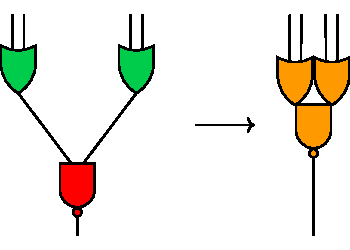
\includegraphics[]{pictures/compiled/einfBsp}
	}
		\caption{Zwei Realisierungen der Logischen Funktion $\neg((w\lor x) \land (y \lor z))$}
		\label{bild:einfbsp}
\end{wrapfigure}
Mithilfe von, aus wenigen Transistoren konstruierten, Bauteilen (genannt Gates, z.B.: AND, OR, INV, OAI) lässt sich eine Logische Funktion nachbilden. Abbildung \ref{bild:einfbsp} (links) zeigt dies an einem kleinen Beispiel.  Die Realisierung einer solchen Funktion ist jedoch nicht eindeutig, wie die in Abbildung \ref{bild:einfbsp} (links und rechts) gezeigte Nachbildung, beweist. \\
Die Größe der Menge aller möglicher Baupläne (später Circuit) für eine Logische Funktion hängt maßgeblich von der Anzahl der zur Verfügung stehenden Bauteile, sowie von dem Aufbau der Funktion, ab.
Es stellt sich heraus, dass im Allgemeinen eine Vielzahl möglicher Realisierungen einer Logischen Funktion existieren. Jedes Bauteil besitzt physikalische Eigenschaften an Größe, Geschwindigkeit (Delay) etc.. Somit besitzt auch jede Realisation solche Eigenschaften. \\
Ziel des \TM ist es für eine Logische Funktion eine Realisierung zu finden, welche eine Kostenfunktion (bestehend aus den physikalischen Eigenschaften) optimiert. Die Wahl der Implementierung hat direkte Auswirkungen auf die  Schnelligkeit, Größe und den Stromverbrauch des fertigen Chips. Hierbei geht das \TM von einer bereits realisierten Logischen Funktion aus und baut diese um zu einer möglichst kostengünstigen Alternative um. \\
Der optimale mögliche Umbau lässt sich bei kleinen oder eingeschränkten gegebenen Bauplänen noch in akzeptabler Zeit finden. Die Lösung dieses Problem für allgemeine Baupläne und Kostenfunktionen ist jedoch ein NP vollständiges Problem. Aus diesem Grund entwickelt die folgende Arbeit eine Heuristik, welche für sehr (mehrere 10.000 Bauteile) große Baupläne in akzeptabler Zeit einen möglichst kostengünstigen Umbau ermöglicht.\\
\textcolor{red}{am ende hier noch eine kurze Quellenübersicht geben an lukas orientiert}

\newpage

\section{Terminologie \& grundlegender Algorithmus}
\label{sec:terminologie&grundl}
\subsection{grundlegende Definitionen}
\label{subsec:grundlegende_definitionen}
Es folgen ein paar grundlegende Definitionen zur Beschreibung des Problems.

\begin{definition}{Boolesche Variable und Funktion: } \\
Eine boolesche Variable ist eine Variable mit Werten in $ \{ 0 , 1 \} $.
Sei $ n, m \in \mathbb{N}$. Eine boolesche Funktion ist eine Funktion $ f : \{ 0 , 1 \}^n \rightarrow \{ 0 , 1 \}^m $ mit n Inputs und m Outputs. 
\end{definition}

\begin{definition}{Gate und Library:}\\
Ein Gate $g$ mit Eingangsgrad $ n \in \mathbb{N}$ ist ein Tripel $(f_g, d_g, area_g)$. Hierbei sind $d_g, area_g \in \mathbb{R}_{\geq 0}$. Des Weiteren gilt $f_g$ ist eine boolesche Funktion mit $ f_g : \{0,1\}^n \rightarrow \{0, 1\} $. \\
Eine Library L ist eine Menge von Gates und sei \\ 
$fanin_{max} := max\{ arity(g) | g \in L \}$.
\end{definition}
\begin{figure}[h]
\begin{center}
 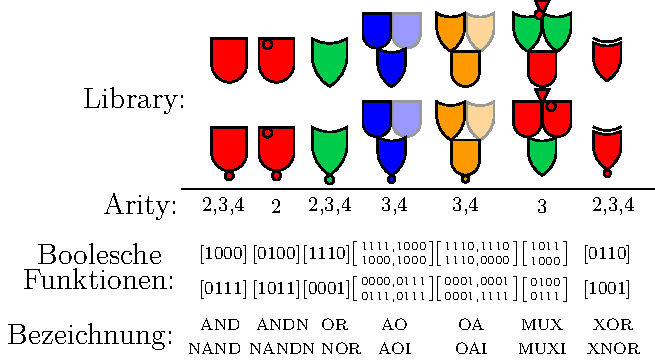
\includegraphics[height = 80pt]{./pictures/compiled/new_library.pdf}
 \caption{Beispiel einer Library}
 \label{bild:new_library}
\end{center}
\end{figure}
$area_g$ gibt die Größe des physikalischen Bauteils an und $d_g$ beschreibt die Zeit die ein Signal braucht um von den inputs des Gates zu seinem Output zu gelangen. Dieser Wert lässt sich noch weiter differenzieren indem man $d_g \in \mathbb{R}^n$ wählt und somit Zeiten für jeden der Inputs angeben werden kann. Hierauf wird jedoch erst in Kapitel \ref{sec:allg_algorithmus} eingegangen. \\
Wenn die Signale der Inputs nicht zur selben Zeit ankommen wird, falls nicht anderes angegeben, gewartet bis das letzte Signal das Gate erreicht.

\begin{definition}{Circuit:}\\
Ein Circuit ist ein gerichteter kreisfeier Graph (directed acyclic graph DAG) mit folgenden Eigenschaften. Jeder Knoten gehört zu einer der aufgelisteten Kategorien: 
\begin{itemize}
\item{\bf Input} Knoten mit Eingangsgrad Null.
\item{\bf Gates} mit mindestens einer eingehenden Kante und ausgehenden Kante. Diese korrespondieren zu der Definition oben mit dem Zusatz dass an jedem der Inputs optional ein Inverter liegen kann.
\item{\bf Outputs} mit genau einer eingehenden Kante und keiner ausgehenden.
\end{itemize}
Ein Gate mit mehr als einer ausgehenden Kante wird auch Highfanoutgate genannt.\\
Ein Circuit realisiert durch Verschachtelung der booleschen Funktionen seiner Gates ebenfalls eine boolesche Funktion. \\
Zwei Circuits heißen äquivalent, wenn sie die gleiche boolesche Funktion realisieren.
\end{definition}

In einem Circuit lassen sich Teilgraphen durch ein Gate der Library austauschen. Voraussetzung für einen solchen Tausch ist, dass der veränderte Circuit äquivalent zu dem originalen ist. Dies formalisieren die folgenden Definitionen. 

\begin{definition}{Match und Kandidat:}\\
Sei g ein Gate in einem Circuit $C$. Ein (invertiertes) Match m ist ein Tupel $(p_m, I_m, f_m, inv_m)$ welches folgendes enthält:
\begin{itemize}
\item Ein Gate p der Library
\item Eine Menge X von Knoten aus der Circuit und eine Bijektion $ f: X \rightarrow inputs(p)$
\item Ein Funktion $ inv : inputs(p) \rightarrow \{not\_inv , inv \}$
\end{itemize}
So dass der Circuit $C'$, welcher durch den Austausch des Sub-Circuits von X bis g durch das Match (mit den durch inv definierten Invertern an den Inputs) entsteht, äquivalent zu C ist.
Ein invertiertes Match auf g ist ein Match auf g mit einem Inverter an jedem seiner Outputs.\\
Ein (invertierter) Kandidat auf g besteht aus einem (invertierten) Match auf g und einem Kandidaten für jeden Input Knoten von g (welcher kein Input von C ist).
\end{definition}

\begin{definition}{Circuit-Kandidat:}\\
Sei C ein Circuit mit Outputknoten Menge O. Eine Circuit-Kandidat K von C ist eine Menge von Kandidaten, sodass $\forall o \in O \, \exists!  h  \in K : h$ ist Kandidat von $ o$ und an jedem Knoten von C an dem sich mehrere Kandidaten überschneiden ist dasselbe Match gewählt.
\end{definition}
Abbildung \ref{bild:grundl_definitionen} visualisiert die vorherigen Definitionen.\\
\newpage
\begin{figure}[h]
\begin{center}
 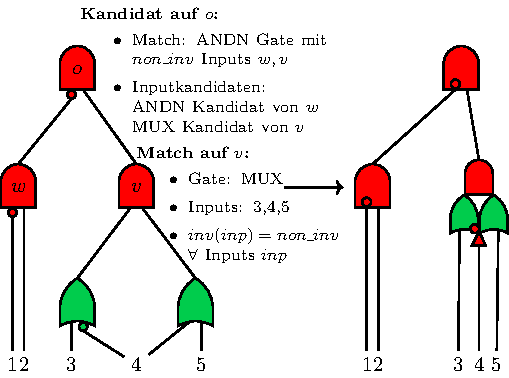
\includegraphics[width = 250pt]{./pictures/compiled/grundl_def_veransch.pdf}
 \caption{Beispiel einer Library}
 \label{bild:grundl_definitionen}
\end{center}
\end{figure}

Ein Circuit-Kandidat C ist eine Möglichkeit den Circuit physikalisch zu realisieren. Wie bereits in der Einleitung bemerkt gilt es nun den besten Kandidaten auf C auszuwählen. Dafür ist ein Maß für Implementierungen von Circuits notwendig. Es folgen zwei geläufige Beispiele. In der Praxis (und im späteren Verlauf dieser Arbeit) wird in der Regel eine convex-Kombination aus beiden verwendet.

\begin{definition}{Area und Delay eines Kandidaten:}\\
Sei C ein Circuit und K ein Circuit-Kandidat auf C. Dann gilt: \\
\begin{itemize}
\item $area(K) = \sum_{g \in gates(C)} (a_g + \sum_{i \in inputs(g)} \mathbb{1}_{inv_g(i)} area_{inv})$ 
\item $AT(K) = $\\$  \max\limits_{k \in can(K)} \{\max\limits_{i \in inputs(k)} \{   d_{gate(k)} + \mathbb{1}_{inv_g(i)} d_{i} + AT(inp\_can(k,i)) + d_{w(k,i)} \} \}$ 
\end{itemize}
Wobei $can(K)$ die Menge der Kandidaten von $K$ sind, $area_{inv}$ die Größe eines Inverters ist und $inputs(k)$ sind die Inputknoten des Outputknoten des Kandidaten k. Des Weiteren ist $d_i$ das Delay eines Inverters und $d_{w(k,i)} $ das Delay der Kante zwischen den Knoten $k$ und $i$. $inp\_can(k,i)$ gibt den Kandidaten des $i$'ten Inputs von k zurück. 

\end{definition}

Das Delay (AT) gibt an, wann das letzte Signal aus einem der Outputs des Circuit kommt.

\subsection{Kern Algorithmus}
\label{subsec:kern_algorithmus}

Es folgt ein grundlegender Algorithmus, welcher auf eingeschränkten Circuits arbeitet, jedoch im weiteren Verlauf dieser Arbeit zu einer Heuristik für allgemeine sehr große Circuits erweitert wird.

\begin{problem}[framed]{(einfaches) Technology Mapping}
  Instanz:  & Circuit $C$ ohne Highfanoutknoten (Knoten mit nur einer ausgehenden Kante), mit eindeutigem Output $o$, Library $L$ mit beschr\"anktem $fanin_{max}$\\
  Aufgabe: &  Finde einen Kandidaten $K$ auf $o$, welcher die Arrivaltime/Area minimiert.
\end{problem}

\begin{algorithm}[H]
 \LinesNumbered
 \DontPrintSemicolon
 \caption{(einfaches) Technology Mapping}
 \SetKwInOut{Task}{Task}
 \KwIn{Circuit $C$ kreisfrei mit finalem Output $o$, Library $L$}

 bester\_kandidat[] $\gets \emptyset$\;
 bester\_inv\_kandidat[]$ \gets \emptyset$\;
 \ForEach{Knoten $v \in V(G)$ in topologischer Reihenfolge}
 {
   berechne alle (invertierten) Matches auf $v$\;
   \ForEach{ Match $m$ auf $v$ }
   {
      Berechne besten Kandidaten mit $m$ auf $v$\;
      Update best\_(inv)\_kandidaten\;
   }
 }
 Implementiere $C$ entsprechend bester\_kandidat[$o$]\;
\end{algorithm}\ \\

\begin{definition}{optimaler \TM Algorithmus:}\\
	Ein Algorithmus für das \TM auf einem Circuit $C$ heißt optimal, wenn er den (bzgl. der Kostenfunktion) besten äquvalenten Circuit $C'$ liefert, welcher durch das Anwenden der erlaubten Operationen auf $C$ konstruiert werden kann. 
\end{definition}
Daraus folgt, dass der Zusatz optimal abhängig davon ist, was die erlaubten Operationen sind.
Im Weiteren Verlauf der Arbeit werden weitere Operationen hinzugefügt und der Circuit verallgemeinert. 
\begin{wrapfigure}{r}{2.8cm}
		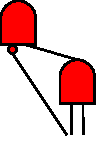
\includegraphics[width = 2.8cm]{pictures/compiled/compl_redundant}
		\caption{Ein Circuit desen boolesche Funktion $f = 0 $ ist}
		\label{bild:compl_redundant}
\end{wrapfigure}
Das Attribut optimal bezieht dann, wenn dies nicht dabei steht,  auf alle bisher vorgestellten Operationen. Zu diesem Punkt umfasst die Menge der erlaubte Operationen das logische äquvalente matchen von Subcircuits mit Elementen der Library.\\

Ein optimaler \TM Algorithmus liefert in der Regel nicht die bestmögliche Implementierung der $C$ zugrunde liegenden logischen Funktion. Dies veranschaulicht Abbildung \ref{bild:compl_redundant}. In diesem Beispiel ist die zugrundeliegende Funktion konstant und somit könnte man auf alle Gates verzichten. Dies ist jedoch mit den bisher eingeführten Möglichkeiten des \TM nicht möglich. \\

\begin{cor}
	Das einfache \TM  ist optimal. 
\end{cor}
\begin{proof}
	Der Algorithmus geht in topologischer Reihenfolge durch die Knoten $v$ des Graphen und berechnet alle Matche auf $v$. Diese werden dann zu einem Kandidaten ergänzt. 
 Ohne Highfanout-Knoten überschneiden sich diese nicht. Für jeden Knoten und jedes Match gibt es nur einen Kandidaten zur Auswahl, da für die Inputs des Matche jeweils nur ein Kandidat gespeichert wurde. An jedem Knoten wird nur das Match (mit dem dazugehörigen Kandidaten) gespeichert, welches die Kosten optimiert. \\
 Es bleibt zu zeigen, dass angenommen für alle Knoten mit kleinerem topologischen Rang als $rand(v)$ ist der bestmögliche Kandidat gespeichert, so wird, nach gerade beschriebenem Vorgehen, auch für $v$ der schnellste (bzw. kleinste) Kandidat $k$ gespeichert. \\
 Angenommen es gibt einen besseren Kandidaten $k'$, als $k$, welcher von dem Algorithmus gespeichert wurde. Sei $k''$ der Kandidate, welcher dasselbe Match wie $k'$ benutzt und die besten Input Kandidaten. Da $k''$ die besten Input Kandidaten benutzt ist er mindestens so schnell (bzw. klein) wie $k'$. $k$ ist jedoch ebenfalls mindestens so kostengünstig wie $k''$ (andernfalls hätte der Algorithmus $k''$, $k$ vorgezogen). Dies ist ein Widerspruch zur Annahme. 
\end{proof}
 
\begin{cor}{Der Algorithmus für das (einfache) \TM  \\ besitzt $\mathcal{O}(  |V(C)|^3|L|^2)$-Laufzeit}
\end{cor}
\begin{proof}
Schritt 1 und 2 besitzen Laufzeit $\mathcal{O}(1)$. Schritt 4 lässt sich, aufgrund von einem beschränkten $fanin_{max}$ und ohne Highfanoutgates, in $\mathcal{O}(|V(C)|^2|L|)$ errechnen. Der Beweis dieser Aussage befindet sich in Kapitel \ref{subsec:match_kandidaten}. Schritt 6 ist, wie bereits erwähnt, schnell implementierbar, da für jeden der max $fanin_{max}$ Inputs nur der beste Kandidat verlinkt werden muss. Ein Invertiertes Match wird nur gebraucht wenn der korrespondierende Input des darüber liegenden Gates invertiert ist. Schritt 6 lässt sich somit in  $\mathcal{O}(fanin_{max})$ realisieren. Schritt 3 und 5 sind zwei verschachtelte Schleifen mit  $|V(C)|$ und max $|L|$ Durchläufen. \\
Daraus folgt eine Laufzeit von $\mathcal{O}(  |V(C)|^3|L|^2)$.
\end{proof}



\newpage
\section{FPTAS und Heuristik}
\label{sec:allg_algorithmus}
\subsection{Tradeoffprobleme}
\label{subsec:tradeoffprobleme}
Der oben vorgestellte Algorithmus ist in der Lage den bestmöglichen Umbau eines eingeschränkten Circuits zu bezüglich Area oder Delay zu errechnen. \\
Es existiert  ein Tradeoff zwischen Area und Delay. Dies hat zur Folge, dass ein möglichst kleiner Circuit im Allgemeinen sehr langsam ist und man bei einer sehr schnellen Lösung mit einem großen Platzverbrauch rechnen muss. In der Anwendung des \TM ist jedoch weder ein sehr langsamer noch ein besonders grosser Circuit akzeptabel.\\
Daraus folgt die Nachfrage nach einem Algorithmus, welcher in der Lage ist bezüglich einer Konvexkombination oder einer Schranke zu optimieren. Daraus ergeben sich die beiden folgenden Optimierungs-Probleme: \\

 \begin{problem}[framed]{\TM mit Konvexkombination}
  Instanz:  & Circuit $C$,mit einem Output, Library $L$ mit beschr\"anktem $fanin_{max}$,
  $|L|$ beschränkt und  Tradeoff-Parameter $\lambda \in [0,1]$ \\
  Aufgabe: &  Finde einen Circuit-Kandidaten $K$ auf $C$, welcher $\lambda AT(K) +(1-\lambda )area(K) $ minimiert.
\end{problem}
 \begin{problem}[framed]{\TM mit Arrivaltimeschranke}
  Instanz:  &  Circuit $C$,mit einem Output, Library $L$ mit beschr\"anktem $fanin_{max}$,
  $|L|$ beschränkt und Arrivaltimeschranke $A_{max}$ \\
  Aufgabe: &  Finde den kleinsten Circuit-Kandidaten $K$ auf $C$, für den $AT(K) \leq A_{max}$ gilt, oder entscheide, dass für jeden Circuit-Kandidaten $K$ bereits $AT(K) > A_{max}$ gilt.
\end{problem}
Im weiteren Verlauf dieses Kapitels, werden diese Problemstellungen auf Circuits mit mehreren Outputs erweitert. \\

Diese \textcolor{red}{diese Probleme sind äquvalent Beweis? oder verweis aus quelle}
\textcolor{red}{erwähnen dass da die äquivalent  nur noch  Konvexkombination}

Dadurch ergibt sich folgende Problemstellung für den Algorithmus: \\
Angenommen an jedem Knoten $v$ würde, wie im Kern-Algorithmus, nur derjenige Kandidat gespeichert werden, welcher die Kostenfunktion an $v$ optimiert. Dadurch kann nicht mehr garantiert werden, dass beim errechnen der Kandidaten für den Output, der für ihn optimale Kandidat noch vorhanden ist. Beide Inputs getrennt nach der Kostenfunktion zu optimieren, garantiert also nicht das optimale Ergebnis.\\

Die Kosten eines Kandidaten k sind somit nicht $\lambda AT(k) +(1-\lambda )area(k)$,  sondern das Tupel $(AT(k), area(k))$.
Es gibt jedoch eine Klasse von Kandidaten, welche nicht gespeichert muss. Dazu folgende Definition\\

\begin{definition}{(dominierte Kandidaten)}\\
	Seien $k_1, k_2$ Kandidaten desselben Knotens. Dann wird $k_1$ von $k_2$ dominiert, wenn mindestens eine der folgenden Bedingungen erfüllt ist.
	\begin{itemize}
	\item $AT(k_1) < AT(k_2) \text { und  }area(k_1) \leq area(k_2)$
	\item $	AT(k_1) \leq AT(k_2) \text{ und } area(k_1) < area(k_2)$	
	\end{itemize}
\end{definition}

 \begin{wrapfigure}{r}{6cm}
		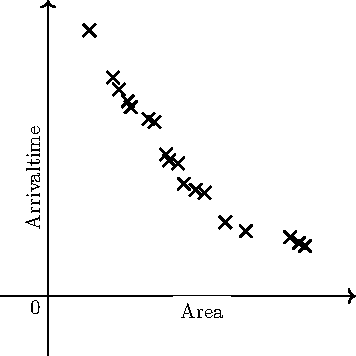
\includegraphics[width = 6cm]{pictures/compiled/tradeoff_kurve}
		\caption{Ordnen der Kandidaten in einer Tradeoffkurve}
		\label{bild:tradeoff_kurve}
\end{wrapfigure}
Eine optimale Lösung des \TM verwendet offenbar (\textcolor{red}{in einem Korollar beweisen ?}) nur nicht-dominierte Kandidaten, woraus folgt, dass nur diese während der Ausführung des Algorithmus gespeichert werden müssen.\\
Die Menge der noch bleibenden Kandidaten lassen sich in sogenannten Tradeoff-Kurven speichern (s. Abb. \ref{bild:tradeoff_kurve}). Welche jeden Kandidaten zweidimensional anhand seiner Kosten erfasst.\\

Die beiden vorgestellten Probleme sind NP-vollständig. Daraus folgt, dass sich ab diesem Punkt wahrscheinlich  kein polynomieller optimaler Algorithmus für das \TM finden lässt. Dadurch dass sich zwei Kandidaten in den meisten Fällen nicht mehr vergleichen lassen, wird eine Vielzahl von Kandidaten an jedem Knoten gespeichert. Dies zeigt sich in einem exponentiell großen Speicheraufwand. \\
Ein Beweis der NP-vollständigkeit findet sich in \textcolor{red}{hier den verweis zu einem Beweis einfügen}.

\subsection{Highfanoutknoten}
\label{subsec:highfanout}
Der oben beschriebene Kern Algorithmus arbeitet nur auf Circuits, in denen keine Highfanoutknoten existieren. Diese Eigenschaft kommt auf einem realen Chip jedoch sehr häufig vor(ca. $30\%$ der gesamten Knoten sind Highfanoutknoten für einen genaueren Zusammenhang von der Anzahl der Highfanoutknoten und der Laufzeit siehe das Kapitel \ref{sec:analyse}).\\
 \begin{wrapfigure}{r}{6cm}
		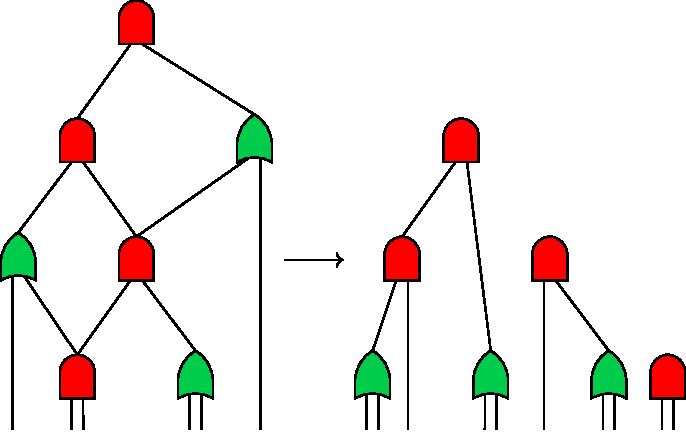
\includegraphics[width = 6cm]{pictures/compiled/ohne_highfanout_heu}
		\caption{Unterteilen eines Circuit in Highfanoutfreie Subcircuits}
		\label{bild:ohne_highfanout_heu}
\end{wrapfigure}
 Es ist möglich einen Circuit, in kleinere Subcircuits zu unterteilen, welche solche Highfanoutknoten nicht besitzen. Die Subcircuits werden einzeln mit dem Algorithmus (sehr schnell) optimiert und daraufhin zu einem C äquivalenten Circuit C' zusammengesetzt. Diese Vorgehensweise findet sich ausführlich in \textcolor{red}{Hier das eine Paper einsetzen} wieder. Abbildung \ref{bild:ohne_highfanout_heu} verbildlicht diesen Ansatz einer Heuristik. 
  Der Anteil an Highfanoutknoten ist auf den mir vorliegenden Chips so groß, dass eine Vielzahl sehr kleiner Subcircuits entsteht, woraus folgt, dass die Möglichkeiten des \TM sehr eingeschränkt werden. Aus diesem Grund werde ich auf diese Art der   Heuristik nicht mehr eingehen.\textcolor{red}{zu anna gibt es sonst noch einen grund dies nicht doch einmal auszuprobieren?}\\

\begin{wrapfigure}{r}{7cm}%[htb]
%\centering
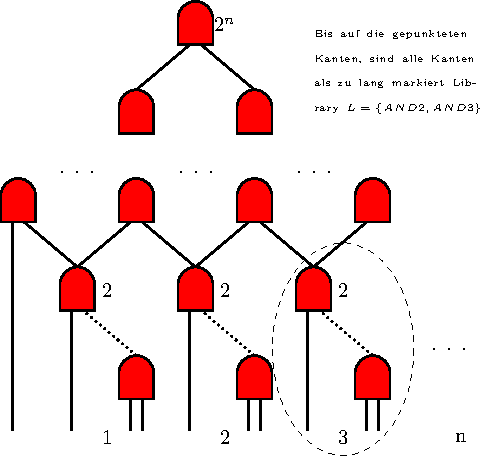
\includegraphics[width= 7cm]{pictures/compiled/expo_kand}
\caption{Exponentiell viele Kandidaten bereits bei sehr eingeschränkter Library}
\label{bild:expo_kan}
\end{wrapfigure}

Das Kern-Problem der Highfanoutknoten ist, dass bei der Konstruktion des äquivalenten Circuits die eingebauten Kandidaten aller Nachfolger eines Highfanoutknoten $v$ an $v$ übereinstimmen müssen. Daraus folgt, das bei der Wahl eines Kandidaten für einen Knoten w die Wahl der Kandidaten der Input-Kandidaten von w nicht unabhängig von einander sein muss. \\
Abbildung \ref{bild:expo_kan} zeigt zudem ein weiteres Problem der Implementierung auf. Die Anzahl der zu Speichernden Kandidaten kann, mit beliebig vielen Highfanoutknoten in $C$,  exponentiell bezüglich $|V(C)|$ sein. Daraus folgt ein Implementierungsproblem, auf welches im Weiteren Verlauf dieser Arbeit noch eingegangen wird. \\
Zur Lösung des ersten Problems helfen die folgenden Definitionen:\\

\begin{definition}{Cone eines Knoten:}\\
	Sei C ein Circuit und v ein Knoten von C. Dann sei die Cone von v: 
	\[ cone(v) := C[V \cup \{ v \}], V = \{ w \in V(C) : \exists \text{ w-v-Weg in }  C \} \] \end{definition}
\begin{definition}\  \\
	Sei C ein Circuit und  $v \in V(C)$. Dann wird die durch $cone(v)$ berechnete Funktion. Die 			{\bf bis v berechnete Funktion} genannt.
\end{definition}

\begin{definition}{Offene Knoten:}\\
	Sei $C$ ein Circuit und $v,w \in V(C)$. Dann heißt $w$ offener Knoten von $v$, wenn folgendes gilt: 
	\begin{itemize}
		\item $ w \in cone(v)\backslash \{ v \} $
		\item $| \delta ^{+}(w)| \geq 2$
		\item $ \exists o \in V(C) \backslash cone(v) : \exists \text{ w-o-Weg in } C \text{ ohne v} $
	\end{itemize}	
\end{definition}
 \begin{wrapfigure}{r}{5.5cm}
		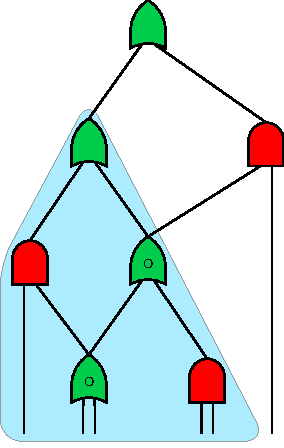
\includegraphics[height = 7cm]{pictures/compiled/cone}
		\caption{Visualisierung der Definitionen 3.2 bis 3.4}
		\label{bild:cone}
\end{wrapfigure}
Mit anderen Worten ist die Menge der Offenen Knoten eines Circuit Knoten $v$, die Menge aller Highfanoutknoten $w$, von welchen aus man sowohl $v$ als auch einen Knoten außerhalb der Cone von $v$ erreichen kann. Von dieser Menge ist $v$ selber ausgenommen. Dies sind gerade die Highfanout-Knoten, welche durch die Kandidaten eines Knoten außerhalb von $cone(v)$ verändert werden können. Alle Kandidaten von  Knoten mit Ausgangsgrad 1 und dieser Eigenschaft, sind durch den Nachfolger-Kandidaten (welcher auch zu einem offene Knoten gehören muss), bereits eindeutig definiert. \\
Abbildung \ref{bild:cone} visualisiert die vorangegangenen Definitionen.\\

\begin{definition}{Klasse eines Kandidaten:}\\
	Sei $k$ ein Kandidat auf einem Knoten $v$ und $O$ die Menge der offenen Knoten von $v$. Die Klasse $class(k)$ ist eine Abbildung, welche jedem Element $w \in O$ den durch $k$ festgelegten Kandidaten auf $w$ zuordnet.\\
\end{definition}
Nach der einführenden Erläuterung lassen sich zwei Kandidaten $k_1,k_2$ eines Knoten $v$ mit $class(k_1) \neq class(k_2)$ nicht miteinander vergleichen. Dies gilt auch für den Fall, wenn $k_2$ von  $k_1$ dominiert wird, denn es ist möglich, dass dies zwar an der Stelle $v$ gilt, jedoch nicht an allen offenen Knoten von $v$. Daraus folgt würde man $k_2$ löschen, so löscht man evtl den besten Kandidaten des Outputs von C. \\
Um somit mit Highfanoutknoten arbeiten zu können, werden für jeden Knoten $v$ und jede Klasse von $v$ ,in dem optimalen Algorithmus, alle nicht dominierten Kandidaten gespeichert. Daraufhin ist der noch verbleibende beste Kandidat des Outputs die beste Lösung.\\
Dabei wird, zur Speicherung der Kandidaten, für jede Klasse eines Knotens eine Tradeoff-Kurve angelegt.

\subsubsection{Klonen}
Oben wurde erwähnt, dass Kandidaten zweier Knoten an den offenen Knoten übereinstimmen müssen. Tun Sie das nicht, so werden offenen Knoten evtl mehrere Male mit verschiedenen Kandidaten gebaut. Dieser Vorgang wird auch Klonen genannt. Dies kann von Vorteil sein, wenn zum Beispiel ein offener Knoten Teil eines sowohl sehr Delay als auch sehr Area kritischen Gebietes ist. Dann würde einmal ein schneller und einmal ein sehr kleiner Kandidat realisiert. Dies führt in der Regel jedoch zu einem deutlich erhöhten Platzverbrauch und es werden mehr Kanten gebraucht, was zu vermeiden gilt. Der erhöhte Verbrauch von Kanten bringt höhere Routing Kosten mit sich, welche im \TM nicht beachtet werden. Um zu verhindern, dass nicht beachtete Ressourcen übermäßig verbraucht werden, Ist das Klonen in den vorgestellten Algorithmen nicht erlaubt und wird durch die Klassen und die Routine, welche beim Verknüpfen von Input Kandidaten zu einem neuen Kandidaten genutzt wird, verhindert. 

\subsection{zu lange Kanten}
\label{subsec:zu_lange_kanten}
 \begin{wrapfigure}{r}{6cm}
		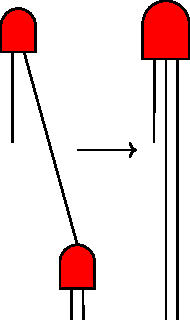
\includegraphics[height = 8cm]{pictures/compiled/zu_lange_kante}
		\caption{Visualisierung eines Matches über eine lange Kante}
		\label{bild:zu_lange_kanten}
\end{wrapfigure}
Abbildung \ref{bild:zu_lange_kanten} veranschaulicht eine häufig auftretende Situation. Es handelt sich das Matchen über eine (auf dem Chip) sehr lange Kante. Dadurch verbessert sich evtl. die Größe des Circuits, jedoch sind nach dem Match nun zwei sehr lange Kanten auf dem Chip vorhanden, was   einen großen Routing Aufwand und weitere Kosten mit sich bringt und somit eine zu vermeidende Situation ist. \\
Weiter unten wird eine zusätzliche Klasse von Kanten eingeführt über welche man nicht matchen darf.
Diese Kanten bezeichet man als konstant.
Um diese Situation zu vermeiden, wird bei der Bildung jedes Matches darauf geachtet über keine konstante Kante zu matchen.\\
Durch die Hinzunahme der zu langen Kanten zu den konstanten Kanten, kann keine optimale Lösung mehr im allgemeinen Algorithmus garantiert werden, von daher wird dies im optimalen Algorithmus nicht gemacht, bei der darauffolgenden Heuristik jedoch schon. \\

 \subsection{Teilweise überflüssige Subcircuits}
 \label{subsec:teilweise_ueberfkl_subcircuits}
 In der Abbildung 4 lässt sich erahnen, dass nicht unbedingt alle Inputs eines Circuits relevant sind für die Outputs. Zur genaueren Einordnung folgt eine Definition.\\
 
 \begin{definition}{vollständig überflüssiger und teilweise überflüssiger Circuit }
 	Sei $C$ ein Circuit mit Logischer Funktion $ f : \{ 0 , 1 \}^n \rightarrow \{ 0 , 1 \}^m $. $C$ wird vollständig überflüssig genannt, wenn gilt:
 	\[  \exists y \in \{0,1 \}^m \forall x \in \{ 0, 1\}^n : f(x) = y  \]
 	$C$ wird teilweise überflüssig genannt, wenn es eine Teilmenge der Inputs gibt, von denen die Signale der Outputs nicht abhängen.
 \end{definition}
 \begin{wrapfigure}{r}{6cm}
		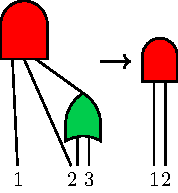
\includegraphics[height = 5cm]{pictures/compiled/partly_redundant}
		\caption{Nur Input 1 und 2 sind die relevanten Inputs}
		\label{bild:partly_redundant}
\end{wrapfigure}
Die Berücksichtigung von vollständig überflüssigen Subcircuits bedeuted, dass Teile des Circuits entfernt werden und die Outputs der Inputs der Nachfolgenden Knoten an permanenten Strom gelegt oder mit der Erdung des Chips verbunden werden.Dies lässt sich jedoch weiter verbessern, da die Information an den Nachfolgenden Gates vorhersagbar ist, muss sie auch nicht verarbeitet werden. Daraus folgt eine hohe Einsparung von Kosten, jedoch birgt es ebenfalls einen großen Aufwand zur Implementierung in der aktuellen Architektur des \TM Algorithmus. In der Praxis ist das Vorkommen von  vollständig überflüssige Circuits verschwindend gering. Von daher werden die vollständig überflüssigen Subcircuits nicht mehr behandelt und kommen auch in den Folgenden Algorithmen nicht vor und zählen auch nicht zu den Kriterien des optimalen \TM. \\
 
Im Gegensatz dazu kommen die teilweise überflüssigen Circuits sehr wohl vor. Bei der Konstruktion eines Chips passiert dies durch das Zusammensetzen unterschiedlicher Circuits.\\
In den meisten Fällen werden die teilweise überflüssigen Circuits automatisch bei der  Suche der Matche gefunden, da die irrelevanten Inputs nicht mehr unter den Inputs des Match auftauchen und somit beim Bau des äquivalenten Graphen verschwinden. Dies veranschaulicht Abbildung \ref{bild:partly_redundant}. \\
Es gibt dabei jedoch noch eine Besonderheit. Wenn alle Inputs bis auf einen Irrelevant sind, so ist das resultierende Gate des Matches entweder ein Inverter(INV) oder ein Buffer(BUFF). Ersteres lässt sich als Input-Invertierung des darüberliegenden Input-Pins speichern. Ein Buffer ist jedoch nicht unbedingt in der Library für das \TM vorhanden und kann vermieden werden. Von daher wird in diesem Fall kein Buffer, sondern nur die Kanten vom Input des Buffers zu seinen Outputs gebaut. Dies verhindert den Einbau eines nicht nötigen Gates. Diese zusätzliche Bearbeitung läuft von nun an in jedem folgenden Algorithmus automatisch im Hintergrund und findet keine Erwähnung mehr.\textcolor{red}{was ist mit dem Laufzeit statistiken?}\\
 Obwohl nun das Gegenbeispiel aus Kapitel \ref{subsec:kern_algorithmus} nicht mehr gültig ist, garantiert auch hier ein optimaler Algorithmus keine bestmögliche Implementierung der eines Circuits zugrunde liegenden logischen Funktion.
 
 
\subsection{Matchingprobleme}
\label{subsec:match_kandidaten}
In Circuits mit beliebig vielen Highfanoutknoten steigt die Anzahl der möglichen Matche eines Knoten sehr stark an, was eine direkte Auswirkung auf die Größe der Menge der möglichen Kandidaten hat. Es folgt eine abstraktere Betrachtung von Matchings und daraus ableitend einen Algorithmus der auf realen Instanzen fast alle möglichen Matche findet und in polynomieller Zeit implementierbar ist.

\subsubsection{Anzahl Matchings}
\label{subsubsec:anzahl_matchings}
Folgendes Lemma legt eine äquivalente Definition für Matche nahe.
Sei, gegeben ein Circuit $C$ ohne teilweise überflüssige Subciruits, \\$\bar{C}_v := (V(C[cone(v)]), \{ (u,v) | (v,u) \in E(C[cone(v)])\})$. 
\begin{lemma}{Die Inputs eines Matches auf $v$ korrespondieren zu den Kanten eines gerichteten $v$-Schnitts in $\bar{C}_v $}
\end{lemma}
\begin{proof}
Zu jedem Inputpin eines Matches gehört eindeutig eine Kantemenge $K$ aus $C$. Es ist möglich, dass $|K| > 1$, denn ein Match kann mehrere ausgehende Kanten eines Knoten zu einer Kante zusammenfasst. Dies veranschaulicht Abbildung \textcolor{red}{??} für ein Match eines MUX Gates.  Sei $I$ die Menge der zu den Inputs korrespondierenden Kantenmengen.\\ 
Es genügt zu zeigen, dass alle Kanten $I'$ in $I$ gerade die Kantenmenge eines gerichteten $v$-Schnitts in $\bar{C}_v$ ist. \\
Angenommen $I'$ bildet keinen gerichteten $v$-Schnitt, dann existiert in $\bar{C}_v\backslash I$ ein Weg von einen Input von $cone(v)$ zu $v$, welcher keine Kante aus $I$ benutzt. \\
Eine Kante dieses Weges muss jedoch zu einem der Inputs des Matches gehören, denn sonst hätte das Match einen Seiteninput, was nicht erlaubt ist, oder es existiert ein teilweise überflüssiger Subcircuit. Daraus folgt die Aussage. 
\end{proof}
Die Korrespondenz ist nicht eindeutig, denn ob mehrere Kanten eines Outputs zusammengefasste oder getrennte Inputkanten eines Matches sind, lässt sich anhand des Schnittes nicht herleiten. Die wird ebenfalls durch Abbildung \textcolor{red}{??} veranschaulicht. Ohne Highfanoutknoten ist diese Zuweisung jedoch, abgesehen von den möglichen Invertierungen der Inputs und des Outputs, eindeutig, wenn es keine zwei Gate der Library gibt, welche diegleiche  logische Funktion realisieren.\\
In einem Graphen ohne Highfanoutknoten gilt somit: 
Die Menge der Matchings von $v$ ist somit gerade die Menge aller, maximal $fanin_{max}$ großen $v$-Schnitte in $\bar{C}_v$, inclusive aller möglicher Inputinvertierungen und Outputinvertierungen, die als Subgraph interpretiert ein Gate der Library realisieren.
\begin{cor}\label{cor:anz_matche_einfach}
Sei $C$ ein Circuit. Die Anzahl der Matche eines Knotens $v\in V(C)$ mit $n_v := |E(C[cone(v)]|$, wobei $C[cone(v)]$ keine Highfanoutknoten enthält, ist durch $n_v^{fanin_{max}} 2^{fanin_{max}+1} fanin_{max}$ beschränkt
\end{cor}
\begin{proof}
Sei  $X_v:= \{ E \subseteq E(C[cone(v)]) | |E|\leq fanin_{max}  \}$. Die Menge der maximal $fanin_{max}$ großen $v$-Schnitte ist in $C[cone(v)]$ durch $ |X_v|$ beschränkt. Es gilt hierbei \[ |X_v| = \sum\limits_{i \leq fanin_{max}} \binom{n}{i} \leq  \sum\limits_{i \leq fanin_{max}}\frac{n}{i!(n-fanin_{max})!} \leq n^{fanin_{max}} fanin_{max} \]
Für jeden Schnitt gibt es noch zwei Verschiedene mögliche Output-Invertierungen und maximal  $2^{fanin_{max}}$ viele Möglichen die Inputs zu Invertieren. Jedes mögliche Match ist nun durch ein Element aus $X_v$ und eine Wahl von Invertierungen eindeutig charakterisiert. Daraus folgt die Aussage.
\end{proof}
Für allgemeinere Circuits lässt sich folgende Schranke angeben. 
\begin{cor}\label{cor:anzahl_matche_bel}
Sei $C$ ein Circuit. Die Anzahl der Matche eines Knotens $v\in V(C)$ mit $n_v := |E(C[cone(v)]|$ mit $\Delta C[cone(v)] \leq fanout_{max}$, enthält, ist durch $n_v^{fanin_{max}} fanin_{max}^22^{fanin_{max}+1}2^{fanout_{max}}$ beschränkt
\end{cor}
\begin{proof}
Korollar \ref{cor:anz_matche_einfach} gibt eine obere Schranke für die Anzahl aller Matche inklusive der möglichen Invertierungen an. Sei $u \in x \in X_v$ (Definition siehe oben) zusätzlich ausgehende Kante eines Highfanoutknoten $w$, so gibt es bis zu $2^{fanout_{max}-1}$ Möglichkeiten weitere Kanten von $w$ der korrespondierenden Kantemenge von $u$ hinzuzufügen.  Diese Möglichkeit besteht für alle maximal $fanin_{max}$ Kanten von $x$. Durch Multiplikation mit der oberen Schranke aus Korollar \ref{cor:anz_matche_einfach} folgt die Aussage.
\end{proof}
In einem Circuit ohne Highfanoutknoten lässt sich die Schranke noch genauer angeben. 
\begin{cor}\label{cor:anz_matche_einfach_genauer}
Sei $C$ ein Circuit ohne Highfanoutknoten. Die Anzahl der Matche eines Knoten ist durch $2^{2fanin_{max} +1}fanin_{max}$ beschränkt.
\end{cor}
\begin{proof}
Ausgehen von einem Knoten $v \in V(C)$ mit maximal $fanin_{max}$ Inputs, gibt es  $2^{fanin_{max}}$ Möglichkeiten die an den Input liegenden Gates mit in das Match einzuschließen. Abgesehen von einer, schließt jede dieser Möglichkeiten mindestens ein Gate mit ein. Da $C$ keine Highfanoutknoten enthält, wird der Fanin des Matches um mindestens eins erhöht, denn es ist nicht möglich Kreise zu schließen. Daraus folgt, dass der obige Schritt maximal $fanin_{max}$ mal durchführbar ist. Für jedes so berechneten Prototyp einen Matches gibt es noch $2^{fanin_{max}}$ mögliche Invertierungen der Inputs und $2$ des Outputs, woraus die obige Aussage folgt.
\end{proof}
\begin{definition}
Sei $\mathcal{M}:= |V(C)|^{fanin_{max}} fanin_{max}^22^{fanin_{max}+1}2^{fanout_{max}}$ eine Bezeichnung der oberen Schranke für die Anzahl der Matche eines Knoten in einem Graphen mit beschränktem $fanin_{max}$ und $fanout_{max}$.
\end{definition}

\subsubsection{Matching Suche in polynomieller Zeit}
Der Kernalgorithmus aus Kapitel \ref{subsec:kern_algorithmus} findet alle möglichen Matche eines beliebigen Knotens in polynomieller Zeit. Dies ist dort möglich, da in dem Circuit keine Highfanoutknoten existieren. Aus Korollar \ref{cor:anz_matche_einfach_genauer} folgt, dass potenziellen Matche aller Knoten  in $\mathcal{O}(2^{2fanin_{max} +1}fanin_{max} |V(C)|)$ errechnet werden können. Da $fanin_{max}$ als Konstante deklariert wurde entspricht dies linearer Laufzeit. Es bleibt zu prüfen ob  ein solcher Prototyp einem Match in $C$ entspricht, also ob die logische Funktion des Subcircuits einem Match der Library gleicht. Für jede der maximal $2^{fanin_{max}}$ möglichen Wahrheitsbelegungen der Inputs wird der Wahrheitsgehalt des Outputs errechnet. Dies ist linear in $|V(C)|$ möglich. Die dadurch errechnete Tabelle wir mit den $|L|$ Gates der Library verglichen. \\
Daraus folgt, dass das Finden aller Matche in $\mathcal{O}(|V(C)|^2|L|)$ und somit polynomiell, möglich ist.

Bei Circuits mit beliebig vielen Highfanoutknoten aber beschränktem $fanout_{max}$, lassen sich durch Korollar \ref{cor:anzahl_matche_bel} und gleichem Vorgehen wie oben alle Matche ebenfalls in polynomieller Zeit finden. Dabei beträgt die Laufzeit $\mathcal{O}(|V(C)|^{fanin_{max}+2}|L|)$.

\subsubsection{heuristische Matching Suche}
In der Praxis, ähnlich dem oben beschriebenen Fall ohne Highfanoutknoten, wird von dem Gate eines Knoten ausgehend überprüft ob dieser, oder eine Mögliche Invertierung, einem Gate der Library entspricht. Daraufhin wird jede der maximal $2^{fanin_{max}}$ Möglichkeiten die an den Input liegenden Gates mit in das potenzielle Match hinzuzufügen inclusive möglicher Invertierungen überprüft. Dieser Vorgang wird für jede der Möglichkeiten so lange wiederholt, bis die Anzahl der Inputs des durch das potenzielle Match,  beschriebenen Subcircuit größer als $fanin_{max}$ ist. Ab diesem Punkt wird das vorliegende Potenzielle Match nicht mehr erweitert. \\
Dies garantiert, bei einem Circuit mit Highfanoutknoten, nicht das Finden aller möglicher Matche, da sobald ein potenzielles Match einen Highfanoutknoten mit einschließt die Zahl der Inputs sinken kann. \\
In der Praxis werden so jedoch die überwiegende Mehrheit der Matche gefunden. Der Verlust einiger weniger Matche spiegelt bringt einen enormen Laufzeitgewinn mit sich.
\textcolor{red}{die dissertation für den fall ohne highfanoutknoten erwähnen ? und nochmal genau durchsehen ob die teilweise überflüssigen Subcircuits überall rausgehalten wurden }


\subsection{Kandidaten-Probleme}
Die Anzahl der Kandidaten an einem Knoten ist im Allgemeinen nicht polynomiell Beschränkt, wie Abbildung \ref{bild:expo_kan} beweist. Dies gilt offenbar auch wenn der Circuit $C$ keine Highfanoutknoten besitzt. Dieses Problem wird durch das Filtern mit Buckets gelöst. Dies wird nach dem Folgenden Korollar eingeführt. 
\begin{cor}
Sei $C$ ein Circuit und $v \in C$. Die Anzahl der Klassen von $v$ ist exponentiell in $k:= |offene\_Knoten(v)|$ beschränkt.
\end{cor}
\begin{proof}
Sei $K$ die größte Kardinalität einer Kandidatenmenge von einem Knoten $w\in offene\_Knoten(v)$. Jede Kombination von Kandidaten der offenen Knoten entspricht, solange sich diese nicht gegenseitig ausschließen, einer Klasse von $v$. Die Anzahl dieser Kombinationen ist durch $K^k$ beschränkt. Daraus folgt die Aussage.
\end{proof}

\subsubsection{Filtern mit Buckets}
\label{subsubsec:filtern}
Die Kandidaten eines beliebigen Knoten sind in Tradeoffkurven, nach Klassen sortiert, gespeichert. Die Werte einer solchen Kurve lassen sich in Abschnitte (buckets) fester Größe einteilen. Dabei lässt sich eine Kurve sowohl in Delay-Buckets  der Größe $\delta_{delay}$, als auch in Area-Buckets der Größe $\delta_{area}$ unterteilen. Dies wird in Abbildung \ref{bild:tradeoff_kurven_filtern} veranschaulicht.\\
\begin{figure}[h]
\centering
\begin{subfigure}{.5\textwidth}
  \centering
  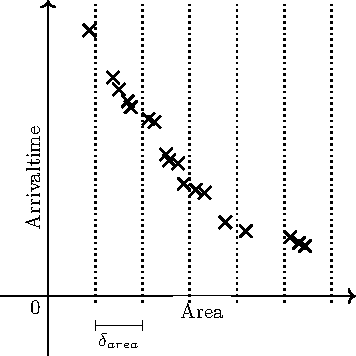
\includegraphics[width=.7\linewidth]{pictures/compiled/tradeoff_kurve_buckets}
\end{subfigure}%
\begin{subfigure}{.5\textwidth}
  \centering
  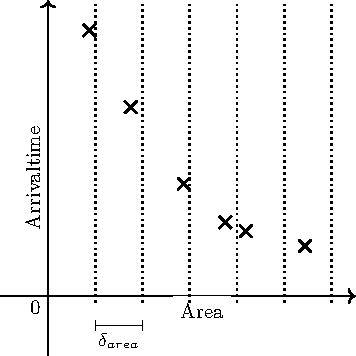
\includegraphics[width=.7\linewidth]{pictures/compiled/tradeoff_kurve_filtered}
\end{subfigure}
\caption{Einteilen und filtern mit Buckets}
\label{bild:tradeoff_kurven_filtern}
\end{figure}
Man wählt die Bucketgrößen $\delta_{area} = \frac{\epsilon}{2(1-\lambda)}, \delta_{delay} = \frac{\epsilon}{2\lambda}$ (mit Tradeoff $\lambda$), und speichert erst nur den kleinsten Kandidaten in jeder Area-Bucket und von den verbleibenden nur den schnellsten in jeder Delay-Bucket.\\
Dadurch ist die maximale Anzahl an Kandidaten in einer Tradeoffkurve polynomiell beschränkt. 
\begin{definition}
Sei $\mathcal{B}$ die maximale Anzahl an Kandidaten in einer Tradeoffkurve, nachdem sie gefiltert wurde.\\
Des Weiteren sei $\mathcal{K}$ die maximale Kardinalität von Klassen eines Knoten.
\end{definition}
\textcolor{red}{M genauer einschränen und die Schranken irgendwo mit hineinbringen bzw beweisen, dass M pol. beschränkt ist. }
\textcolor{red}{was ist mit dem beweis ? kann ich lukas verlinken oder verlinkt der auf irgendwen ?}

Beschränkt man die maximale Anzahl von Highfanoutknoten in $C$, so folgt aus dem obigen Korollar, dass die Anzahl der Klassen eines jeden Knoten und die Menge der sich darin befindlichen Kandidaten, polynomiell beschränkt ist. \\
Aus diesem Grund geht der im Folgenden vorgestellte polynomielle Algorithmus von einer beschränkten Anzahl von Highfanoutknoten aus.\\ 

Es folgt ein kurze Beschreibung, wie die Kandidatemenge eines Knoten gebildet wird.

\subsubsection{Verknüpfen von Kandidaten}
Ohne Highfanoutknoten lassen sich bei der Konstruktion eines Kandidaten für einen Knoten $x$, die Kandidaten $k_i$ der Inputs $i$ unabhängig voneinander wählen.
Da das Klonen nicht erlaubt ist, ist dies bei Circuits mit erlaubtem höheren Fanout nicht möglich.\\
Die folgenden Bedingungen stellen sicher, dass Klonen verhindert wird. \\
Seien für einen Knoten $v$, $O_v$ die Menge seiner offenen Knoten.
\begin{itemize}
	\item[1.] $\forall v,w \in Inputs(x) \forall y \in O_v \cap O_w : class(k_v)(y) = class(k_w)(y)$
	\item[2.] $\forall v,w \in inputs(x) \text{ mit } v \in O_w : k_v = class(k_w)(v)$
\end{itemize}
Bedingung 1 stellt sicher, dass die an den offenen Knoten der Inputkandidaten ein eindeutiger Kandidate festgelegt wird. Bedingung 2 sichert diese Eigenschaft auch für die Inputs selber, denn es ist möglich dass ein Inputknoten von $x$ auch ein offener Knoten eines weiteren Inputs ist. Für diesen wird dadurch ebenfalls ein eindeutiger Kandidat festgelegt. \\
Somit sind alle Inputkandidatenmengen, welche diese beiden Bedingungen erfüllen, eine mögliche Grundlage für einen Kandidaten auf $x$. 

\subsubsection{Finden von Kandidaten} 
Für jedes der maximal $\mathcal{M}$ Matche eines Knoten $v$ von einem Circuits mit den oben genannten Einschränkungen gilt folgende Vorgehensweise zur Findung aller passender Kandidaten. Jedes Match $m$ besitzt höchstens $fanin_{max}$ Inputs. Sei $K_i$ die Menge der Klassen von Input $i$ des Matches. Jedes Element aus der Menge der möglichen Klassen $\prod_{i\leq |inputs(m)|} K_i $ wird auf die obigen Bedingungen überprüft. Die Kombinationen $O$, welche beide Bedingungen erfüllen bilden eine Klasse von $v$. In die  dazugehörige Tradeoffkurve kommt nun jede nicht dominierte Kombination von Kanidaten der Tradeoffkurven von $O$. \\
Die lässt sich in Laufzeit $\mathcal{O}(\mathcal{M}(\mathcal{KB})^{fanin_{max}} )$ implementieren. Da alle Elemente dieser Formel polynomiell beschränkt sind, entspricht aus dies polynomieller Laufzeit.
 
\subsection{FPTAS}
\label{subsec:fptas}
Erweitert man Circuits um die bisher in diesem Kapitel beschriebenen Eigenschaften, beschränkt durch $k$-Highfanoutgates. So gibt es für das folgende Problem einen FPTAS(Fully polynomial time approximation scheme). Ein FPTAS ist ein Algorithmus, welcher, gegeben ein $\epsilon > 0$, eine Lösung des Problems errechnet mit der Eigenschaft, dass für deren Kosten $c \leq (1+\epsilon)OPT$ gilt. \\
 \begin{problem}[framed]{FPTAS für das \TM}
  Instanz:  & Circuit $C$ mit einem Output, Library $L$ mit beschr\"anktem $fanin_{max}$, maximal $k$ Highfanoutknoten, Tradeoffparameter $\lambda \in [0,1]$, Toleranz $\epsilon > 0$ \\
  Aufgabe: &  Finde einen Circuit-Kandidaten $K$ auf $C$, mit Kosten $c \leq (1+\epsilon)OPT$.
\end{problem}
\textcolor{red}{algorithmus und laufzeit einfügen}\\
{\bf Laufzeit: }
\textcolor{red}{hier kommt die anahme der polynomiellen laufzeit hin diese hier grob beschreiben. bei den überflüssigen Circuits kann man darauf eingehen, dass die ohne diese auch polynomiell ist man könnte dafür die überflüssigen subcircuits auch einfach vorziehen. dann wird der tiel leichter}\\
\textcolor{red}{Laufzeit des FPTAS}

\subsection{Heuristik}
\label{subsec:heuristik}
Im folgenden Algorithmus ist die Menge der Knoten mit $fanout > 1$ beliebig groß.
Die Anzahl der Highfanoutknoten bestimmt maßgeblich den Speicherbedarf an Kandidaten und Laufzeit des FPTAS. Sie sind der Grund, warum sich der FPTAS für eine Anwendung des \TM auf einem gesamten Chip nicht eignet. \\
Von daher ist es ein naheliegender Ansatz für eine Heuristik, an jedem Highfanoutknoten nur einen Kandidaten zu speichern. Es ist jedoch nicht trivial, welchen man dort auswählt. Die Auswahl eines solchen Verfahrens wird in Kapitel \ref{sec:premapping} ausführlich behandelt. Im Folgenden wird Beipielhaft eines dieser Verfahren erläutert. \\
Ist an jedem Highfanoutknoten ein Kandidate gewählt, so lässt sich der noch bestmögliche Circuit Kandidat schnell errechnen, da für jeden Knoten nur eine Klasse (und Tradeoffkurve) vorhanden ist.\\
\begin{algorithm}[H]
 \LinesNumbered
 \DontPrintSemicolon
 \caption{Heuristik f\"ur das TM mit Konvexkombination}
 \SetKwInOut{Task}{Task}
 \KwIn{Circuit $C$ mit finalem Output $o$, Library $L$, $\lambda \in [0,1], \epsilon >0$}
 \ForEach{Knoten $v \in V(C)$}
 {
  berechne Matche für $v$\;
  lösche alle konstante Kanten überdeckende Matche für $v$\;
  berechne alle nicht dominierten Kandidaten auf $v$\;
  \If{$v$ ist Highfanoutknoten}
  {
    $guess \gets \min\limits_{\text{Kandidat }k\text{ auf }v}\{ \lambda AT(k) + (1-\lambda) area(k)  \}$\;
    \ForEach{Kandidat $k$ auf $v$}
    {
      \If{$k \neq guess$}
      {
	l\"osche $k$\;
      }
    }
  }
  filter\_kandidaten\_mit\_buckets$(v,\epsilon)$\;
 }
 Baue $C'$, ohne Buffer, entsprechend des besten Kandidaten auf $o$ \; 
\end{algorithm}\ \\

Schritt 2 berechnet evtl. nicht alle möglichen Matche. Die Routine zur Matching Suche, geht von einem Knoten aus und zieht solange Gates mit in das Match, bis $fanin_{max}$ überschritten wird \textcolor{red}{ach scheiße mach mal eine vernünftige laufzeit für das Suchen der Matche pack das aber in Das kapitel oben drüber rein}
Schritt 5-9 beschreibt ein einfaches Verfahren zur Auswahl eines Kandidaten für einen Highfanoutknoten. Angelehnt an den Kernalgorithmus wir nur der Kandidate behalten, welcher den Tradeoff minimiert. Dies garantiert keine optimale Lösung. Weitere Informationen befinden sich in Kapitel \ref{sec:premapping} und \ref{sec:analyse}. \\
{\bf Laufzeit: } Die Schleife aus Schritt 1 läuft durch alle Knoten. Die Laufzeit für Schritt 2 wurde bereits erläutert und Schritt 3 ist Linear in der Anzahl der gefundenen Matche implementierbar. \\
Schritt 4 hat einen Laufzeit von \textcolor{red}{auch hier eine Laufzeit angeben!!! kümmere dich mal um die maximale Anzahl Matches, Kandidaten und die Laufzeiten um diese zu finden und mach ein kapitel draus }\\
Schritt 10 ist linear in der Anzahl der Anzahl der Kandidaten pro Knoten und Schritt 11 linear in der Menge Kandidaten pro Knoten und $|V(C)|$.\\
Daraus folgt eine Laufzeit von \textcolor{red}{hier hin damit!}



\section{Mehrere Outputs}
Bisher wurde auf Circuits $C$ mit nur einem Output gearbeitet. Reale Instanzen eines Chips sind jedoch mit beliebig vielen Outputs ausgestattet. Outputs können auch zusätzlich noch Nachfolger in $C$ besitzen. Da Signale dieser Knoten ebenfalls aus der Cone darüberliegender Knoten laufen können, werden sie ebenfalls als offene Knoten ihrer Nachfolger deklariert. Des Weiteren ist in einem Ciruit mit mehreren Outputs AT alleine ein schlechtes Optimierungskriterium. \\
Des Weiteren sind viele Gates, zumindest teilweise, symmetrisch aufgebaut (Bsp. AND, OR) und die Signale der Inputs brauchen unterschiedlich lange zum Output des Gates. Daraus folgt, dass durch Permutierung von Teilmengen der Inputs Geschwindigleitsvorteile geschaffen werden können. 
\textcolor{red}{oder das kommt unter weitere Optimierungskriterien, dass dieses Kapitel mehrere Outputs heissen kann und die Optkriterien nicht so leer sind}
\subsection{required Arrivaltimes}
\label{subsec:rat}
Oben wurde bereits der Begriff der Arrivaltime eines Knoten eingeführt. Dies ist die Zeit, zu welcher das letzte Signal bei einem Knoten ankommt. Diese Werte sind für die Inputknoten eines Circuits $C$ gegeben und werden von dort aus (unter Hinzunahme von Wire-, Gate- und Inverter-Delay) für jeden Knoten von $C$ (in topologischer Reihenfolge) errechnet.\\
Im Design Prozess eines Chips, gibt es neben der tatsächlichen Arrivaltime auch eine  gewünscht Arrivaltime RAT (required AT), welche an den Outputs eines Graphen gegeben ist und ähnlich zur AT durch C propagiert wird. Somit ist sowohl AT und RAT eine Funktion auf $V(C)$. \\
Der Vollständigkeit wegen folgt hier nocheinmal die genaue Definition der RAT.\\

\begin{definition}{RAT:}\\
	Sei $C$ ein Circuit und $v \in V(C)\backslash  Outputs(C)$. Die RAT (required arrivaltime) an v ist definiert durch:
	\[   RAT(v) := \min\limits_{ \substack{(v,x)\in E(C), \\ i: inputs(x)[i] = v }} \{ RAT(x) - d_{w(v,x)} - d_{gate(x)} - d_{i} \mathbb{1}_{inv_x(i)} \}\] 
	Die RAT der Outputs wird hierbei (wie das Delay der Inputknoten) als gegeben angenommen. 
\end{definition}

In der Praxis kommen Signal oft später an als gewünscht. Der Betrag des Slack $slack(v) := RAT(v) - AT(v)$ gibt, wenn $slack(v) \leq 0 $, an um wie viel Zeit sich das letzte Signal an $v$ verspätet. Somit ist es viel Interessanter einen gegebenen Circuit hinsichtlich des negativen Slacks zu verbessern. \\
Hieraus ergeben für einen Circuit die beiden folgenden Werte: 
\begin{itemize}
	\item Worst-Slack (WS): Wert des kleinsten Slacks für einen Knoten auf dem Circuit.
	\item Sum-of-Negative-Slacks (SNS): Summe aller negativer Slacks der Outputs eines Circuits.
\end{itemize}
Letzteres ist in der Praxis gefragter, da eine sehr gute Verbesserung der SNS eine Verbesserung des WS in der Regel mit einschließt. \\

\textcolor{red}{hier passt sehr gut rein Lukas FPTAS zu erwähnen da er auf den schlechtesten Pfad angewendet wird, war die anzahl der Highfanout gates vorhersebar? -> in den nächsten absatz mit einbauen}\\

Angenommen man betrachtet einen Chip, dann lässt sich auf diesem ein Knoten $v$ finden, an welchem der WS angenommen wird. Sei $C$ der Circuit, welcher nur aus dem Gate von $v$ besteht. Füge nun zu $v$ in $C$ den Input von $v$ hinzu, welcher den größten negativen Slack besitzt. Dies wiederhole man für das neu hinzugefügte Gate, bis man an einem Input des Chips gelangt oder der Slack nicht mehr negativ ist. \\
Hieraus entsteht ein Circuit $C$ welcher einen Output hat und aus einer hintereinangeschalteten Kette von Knoten besteht. Dieser lässt sich nun mit geeigneten Algorithmen \textcolor{red}{füge hier mal ein Beispiel oder einen Verweis an} zu einem äquvalenten Circuit C', mit geringerer Tiefe(\textcolor{red}{schon definiert(wenn nein nötig?)}, umformen. Dieser lässt sich dann mit  Delay optimierenden \TM (in polynomieller Laufzeit\textcolor{red}{zeigen ?}) umbauen und wieder in den Chip einbauen. Der Große Vorteil von diesem Vorgehen sind überschaubar große Instanzen und eine Beschleunigung des gesamten Chips in sehr schneller Zeit. Der Nachteil jedoch ist, dass ein Chip oft sehr viele Wege besitzt, welche einen schlechten Slack realisieren und man somit den Chip nur inkrementell beschleunigt.\\

Eine weitere Herangehensweise für das \TM ist es einen Circuit dahingehend zu optimieren, dass die SNS des Outputs minimiert wird. Dies ist jedoch bei den bisher betrachteten Circuits äquivalent zur Optimierung nach AT, da nur Instanzen mit einem Output betrachtet wurden und RAT für diesen eine Konstante ist.

\subsection{Mehrere Outputs}
\label{subsec:mehrere_outputs}
Wie in der Einleitung beschrieben, ist es das Ziel dieser Arbeit eine Heuristik für das \TM zu entwickeln, welche auf großen Teilen eines Chips lauffähig (bezüglich Laufzeit) ist. Da ein solcher Chip mehr als nur einen Output-Pin besitzt, lässt er sich in zusammenhängende Circuits unterteilen, welche mehr als einen Output-Knoten besitzen. Folgende Umbauten sind notwendig um mit den Kern-Algorithmus auch diese Instanzen verbessern zu können.\\

Als erstes fällt auf, dass sich, wenn der Algorithmus für jeden Knoten die Kandidatenmenge errechnet hat, nicht einfach der beste Kandidat für den Output aus seiner Tradeoff-Kurve auswählen lässt. Dieser besitzt bei mehreren Outputs nämlich In der Regel offene Knoten. 
Jedoch ist bereits bekannt wie man mehrere Kandidaten auswählt, sodass diese sich an den sich überschneidenden Knoten gleichen. Somit lässt sich ein Circuit mit den bekannten Mitteln ein Circuit konstruieren, welcher eine Kostenfunktion hinsichtlich Größe und WS optimiert. \\

Die zweite Änderung hat sich dadurch bereits angekündigt. Bisher wurde das Delay eines Circuits C optimiert, indem das Signal des einen Outputs nach dem Umbau früher ankommt. Dies lässt sich auf einen Circuit mit mehreren Outputs übertragen. Da es mehrere Signale gibt wählt man den Kandidaten des Outputs mit dem größten negativen Slack zuerst und die anderen folgen sortiert der Größe ihres Slacks nach (absteigend). Dies garantiert jedoch nicht, dass der WS des Circuits nach dem Umbau besser ist als vorher, da evtl der Knoten der vorher den WS bildete besser wird, jedoch ein anderer Output könnte durch diesen Umbau schlechter werden. \\
Um dieses Problem zu umgehen, verändert man C vor dem \TM durch das verbinden aller Outputs mit einem virtuellen Gate, mit nur einem möglichen Match (dem Gate an sich). Der veränderte Circuit lässt sich nun wie im Kern-Algorithmus optimieren und es wird automatisch das gerade beschriebene Problem gelöst.\\ 
Wie bereits in Kapitel \ref{subsec:rat}  erwähnt ist es in der Praxis profitabler die SNS des Circuits zu verbessern, anstatt den WS.\\
Also muss aus den Kandidatenmengen der Outputs derjenige Circuit-Kandidat gebaut werden, welcher die SNS minimiert.\\
 Dieses Kriterium ersetzt, von diesem Punkt an,  das der Delay-Optimierung in der Kostenfunktion.\\
 
 Des Weiteren müssen nach dem \TM noch alle Outputs, mit der bis zu ihnen realisierten Logischen Funktion, vorhanden sein. Daraus folgt, dass über einen Output-Knoten, welcher in dem Circuit noch mindestens einen Nachfolger hat, nicht gematcht werden darf, denn sonst würde ein nicht erlaubter Seitenoutput entstehen.\\
 Die lässt dadurch bewerkstelligen, dass man eine seiner ausgehenden Kanten als konstant deklariert, wie das bereits bei den zu langen Kanten geschehen ist. 

 \textcolor{red}{ indem unterkapitel noch mehr bilder bzw schönerer aufbau ist nämlich aktuell viel text!!}
 
\begin{comment}
 \subsection{Allgemeiner Algorithmus}
 \label{subsec:allg_algorithmus}
 
\textcolor{red}{\huge das kommt weg bzw in ein Kapitel was die Heuristik erweitert und eine neue Laufzeit angibt} 
 
 
 
 \textcolor{red}{beschreibe hier evtl nur die Veränderungen der Implementierung die hier vorgenommen werden müssen um Multiple otuputs zu integrieren also reichen eigentlich wenige sätze des weiteren muss der quatsch mit dem optimalen TM zum als konkreter Algo mit laufzeit verschwinden, da nicht interessant}
 Es folgt ein optimaler  \TM Algorithmus welcher auf allgemeinen Circuits arbeitet. 
 \textcolor{red}{TODO Laufzeit  und Korrektheitsbeweis? was ist mit dem faninmax ? vielleicht nett zur laufzeit berechnung aber eig hier noch nicht relevant   erwähnen woraus die kostenfunktion besteht bzw nur tradeoffparameter nehmen!!!!}\\
 \textcolor{red}{hab ich schon erwähnt wie man Kandidaten auswählt ?}
 
 \begin{problem}[framed]{(allgemeines) Technology Mapping}
  Instanz:  & Circuit $C$, Library $L$ mit beschr\"anktem $fanin_{max}$\\
  Aufgabe: &  Finde einen Circuit-Kandidaten $K$ auf $C$, welcher die Kostenfunktion c minimiert.
\end{problem}

\begin{algorithm}[H]
 \LinesNumbered
 \DontPrintSemicolon
 \caption{(allgemeines) \TM}
 \SetKwInOut{Task}{Task}
  \KwIn{Circuit $C$,  Library $L$, $fanin_{max}$}
 \ForEach{Knoten $v \in V(C)$ in topologischer Reihenfolge}
 {
 	$tradeoff\_curves[v][] \gets \emptyset$ \;
 	berechne die offenen Knoten $O$ von $v$\; 
 	$classes[v] \gets get\_all\_classes(v,C,  O, tradeoff\_curves)$\;
 	berechne alle (invertierten) Matche auf $v$\;
	\ForEach{ Match $m$ auf $v$ }
  	 {
   		\ForEach {$A \in classes[v]$}
   		{
   				\ForEach {Kandidat $k$ von $v$ mit $m$, der A respektiert}
   				{
   					$ dom \gets k.is\_dominated(tradeoff\_curves[v][A])$\;
					\If {$!dom$}
						{$tradeoff\_curves[v][A].push\_back(k)$}
   				}
   		}
   	}
 }
 $K \gets best\_circuit\_candidate(tradeoff\_curves, C.outputs, c)$\;
\Return K
\end{algorithm}\ \\
 
{\bf Korrektheit:} \\
Es gilt zu zeigen, dass dies ein optimaler Algorithmus ist. \\
Der Algorithmus speichert für jeden Knoten alle, bis auf die dominierten, möglichen Kandidaten. Daraus folgt, dass in Schritt 12 zur Auswahl des besten Circuit-Kandidaten, jeder mögliche nicht dominierte Umbau zur Verfügung steht und dort nur der kostengünstigste, bezüglich c, ausgewählt wird. 
 
 
 \textcolor{red}{ TODO vergleich mit Lukas und geeignete Quellen einfügen!! besonders für den Hautalgorithmus wie bei Lukas nach welchem Vorbeild der entstanden ist}\\
 
 {\bf Laufzeit:} \\
Da, wie bereits oben erwähnt, das \TM auf allgemeinen Circuits ein NP-vollständiges Problem ist, folgt, dass es unwahrscheinlich ist mit diesem Algorithmus größere Instanzen, in aktzeptabler Zeit, lösen zu können. \\
Die Anzahl der Durchläufe der ersten Schleife sind $|V(C)|$. Die Schritte 2,3 und 5 sind ebenfalls in $\mathcal{O}(|V(C)|)$ errechenbar. \textcolor{red}{genaue werte und begründung angeben angeben!} \\ 
Des Weiteren gilt, dass die Schleife aus Zeile 6 für jeden Knoten maximal $2|L|$ mal aufgerufen wird. \\
Die Anzahl der Kandidaten steigt, dank der beliebigen Anzahl an Highfanoutknoten exponentiell, weshalb die Größe von $classes$ und die somit auch die Schleifendurchläufe in Zeile 7 nur polynomiell begrenzt sind. Daraus folgt sowohl eine nicht polynomielle Laufzeit als auch eine nur exponentiell beschränkte Größe des verbrauchte Speichers. \textcolor{red}{genauer?}.\\

Folgende Abbildung veranschaulicht das exponentielle Wachstum der Kandidatenmenge, indem für jeden Knoten die Anzahl der Kandidaten in Verbindung mit seinem topologischen Index angibt. \textcolor{red}{hier Beispielbild mit beschriebenen eigenschaften} \\

\end{comment}


 \section{Premapping von Highfanoutknoten}
 \label{sec:premapping}
Der exponentielle Anstieg der Kandidatenmenge wird, wie oben gezeigt, durch die Highfanout-Knoten verursacht. Daraus folgt, dass ein sehr großes Laufzeit Potenzial in der Reduzierung der Kandidaten für diese Knoten liegt. \\
 Die Kandidatenmenge eines jeden Highfanoutknotens wird, wie bereits in Kapitel \ref{subsubsec:heuristik} geschehen, auf eins reduziert. Diese Routine wird auch das Premapping der Highfanoutknoten genannt. Dadurch folgt, dass jeder Knoten des Circuits $C$ nur noch eine Klasse an Kandidaten besitzt, denn alle offenen Knoten seiner Cone sind Highfanoutknoten und somit festgelegt.  Die Kandidatenmenge der Outputs, welche noch Nachfolger $o \in C$ haben, wird ebenfalls auf einen Kandidaten reduziert. Dies verhindert das Klonen in $cone(o)$, da  auch die nicht offenen Knoten von $o$ von allen Knoten der Menge $O := \{ v \in Outputs(C): o \in cone(v) \}$ mit einem Kandidaten belegt werden.\\
Nun lässt sich der bestmögliche Kandidate eines jeden Outputs, ohne Nachfolger, finden, indem die einzige verbleibende Tradeoffkurve nach dem Kandidaten mit den geringsten Kosten gesucht wird. Dadurch ist das Finden des noch bestmöglichen Circuit Kandidaten ohne Laufzeiteinbußen möglich. \\
Daraus folgt, dass der zu wählende Circuit-Kandidat eindeutig ist, sobald jedem Highfanoutknoten ein Kandidat zugewiesen wurde. Dadurch hat die Wahl der Premapping Routine eine zentrale Bedeutung der Heuristik.\\
Im folgenden werden drei verschiedene Routinen vorgestellt und auf ihre Eigenschaften eingegangen. Genauere Informationen über die Unterschiede der Resultate dieser Routinen finden sich in Kapitel \ref{sec:analyse}.

\subsection{triviales Premapping}
\label{subsec:triviales_premapping}
Diese Methode des Premappings wurde bereits in Kapitel \ref{subsubsec:heuristik} benutzt. Hierbei wird für jeden Knoten folgender Kandidat ausgewählt: \[ guess \gets \min\limits_{\text{Kandidat }k\text{ auf }v}\{ \lambda AT(k) + (1-\lambda) area(k)  \} \]
Diese Methode liegt nahe, lässt sich jedoch noch weiter verbessern. \\
Die garantiert optimale Lösung findet das triviale Premapping jedoch nur mit Tradeoff $\lambda \in \{ 0,1 \}$ 
 
 
\subsection{erweitertes Premapping}
\label{subsec:erweitertes_premapping}
\textcolor{red}{gilt es noch zu entwickeln} 
 
 
\subsection{Premapping durch Schätzen}
\label{subsec:neinhierfrnochkeinlabel}
 Beim Premapping durch schätzen wird versucht eine Vermutung für die Kosten eines guten Kandidaten aufzustellen. Ausgewählt wird dann der Kandidat, welcher die geringste Differenz zu den vermuteten Kosten besitzt.\\
 Die Schätzung erfolgt durch zwei \TM Läufe. Das \TM wird mit demselben Circuit  und den Tradeoff Parametern $0,1$ gestartet.\textcolor{red}{das ist eine gute abschätzung weil man durch die langsame implementierung des kleinen circuits kosten in der Rat bekommt plus die Methode aus Lukas heuristik entnehmen und dazupacken}


\section{Präprozessing}
Die Möglichkeiten des Matchings sind im allgemeinen Vielfältig, jedoch bei Gates $p$ mit $|inputs(p)| = fanin_{max}$ auf das beliebige Invertieren der Inputs und des Outputs beschränkt. \\
Um diesem Problem aus dem Weg zu gehen, ist es möglich vor dem \TM Algorithmus jedes Gate mit mehr als zwei eingehenden Inputs durch einen kleinen Subcircuit bestehend aus zwei Input Gates zu ersetzen. Dies ist immer möglich, da jede Logische Funktion nur mithilfe von NAND2 und INV Gates realisierbar ist (\textcolor{red}{beweis verlinken ?} und auf jedem realen Chip standartmäßig ein AND oder NAND sowie ein OR oder NOR in der Library vorhanden sind. INV Gates sind fester Bestandteil jeder realen Library.\\
Dabei werden die Gates nach folgender Routine zerlegt. \textcolor{red}{hier das huffman coding und ein Beispiel mit einbringen und decomposing begriff einführen}\\
Der Vorteil des Decompose ist, dass die Möglichkeiten des \TM deutlich erweitert werden. Jedoch werden für ein AND4 Gate Beispielsweise 3 AND2 Gates eingesetzt, was dazu führt, dass sich im Allgemeinen die Kosten des Augangscircuits verschlechtern.\\
Eine ausfürhliche Analyse der Vor- und Nachteile des decomposen finden sich in Kappitel \ref{sec:analyse}.
	

\section{Weitere Optimierungskriterien}
Das \TM arbeitet im Chip-Design auf realen Instanzen. Dadurch kommen, zu den bereits vorgestellten, weitere Optimierungskriterien hinzu. Es handelt sich hierbei einmal um Ressourcen, welche in die Kostenfunktion mit eingebracht werden können und somit während des \TM optimiert werden. Des Weiteren verursacht der neu implementierte Circuit Kosten welche im \TM nicht beachtet wurden, für die es jedoch einen übermäßigen Anstieg zu vermeiden gilt. Ein Beispiel hierfür sind die bereits erwähnten zu langen Kanten. Weitere Kriterien folgen. 
\subsection{pinabhängiges Delay}
\label{subsec:pinabh_delay}
Bis zu diesem Punkt war das Delay eine Gates als eine nicht negative Reelle Zahl definiert. Die meisten Gates besitzen mehr als einen Input. Die Signale der Inputs brauchen nicht alle dieselbe Zeit um zum Output zu gelangen. Physikalisch werden die Signale der Inputs zwar alle miteinander verrechnet, jedoch geschieht dies nicht gleichzeitig und somit müssen nicht alle Signale zur selben Zeit an den Inputs anliegen.\\
Die spätere Ankunftsmöglichkeit lässt sich durch einen kleineren Delaywert, spezifisch für diesen Input, realisieren. Denn wenn das Signal schneller durch das Gate gelangen kann, so brauchst es auch nicht so früh vorhanden zu sein, wie die anderen. \\
Von nun an ist das Delay eines Gates $g$: $d_g \in \mathbb{R}_{\geq 0}^{arity(g)}$. Für das \TM ist dies eine weitere Möglichkeit der Verbesserung, denn viele Gates der Library besitzen mindestens eine Teilmenge von Inputs welche logisch symmetrisch aufgebaut sind. Diese lassen sich beliebig permutieren. Durch die unterschiedlichen Delay-Eigenschaften der Inputs kann eine solche Permutierung das Dealy des Outputs verbessern. Aus diesem Grund ändert sich die AT eines Knotens wiefolgt: 
\begin{definition}{AT mit pinabhängigen Delay:}\\
	Sei $C$ ein Circuit und $v \in V(C)$. Die AT von $v$ mit pinabhängigen Delay ist wiefolgt definiert: \[ AT_p(v) :=  \max\limits_{i \in inputs(v)} \{   d_{gate(v),i} + \mathbb{1}_{\{inv_g(i) \}} d_{i} + AT_p(i) + d_{w(k,i)} \}   \}\]
\end{definition}
Im Folgenden sei mit AT immer das pinabhängige Delay gemeint.

In einem Match ist diese Information bereits abgespeichert, da die Inputs eines Matches mit einer Bijektion an Knoten des Circuits geknüpft werden. Um die Optimilität des, noch vorzustellenden, allgemeinen Algorithmus zu wahren, wird ein Kandidat für jede mögliche Permutation der Inputs gespeichert, falls dieser nicht dominiert ist.\\
Nach aktuellen Stand gilt $fanin_{max} \leq 4$. Das ist klein genug um auch bei der Heuristik die max $fanin_{max}$ Permutation bei der Wahl eines Matches in Betracht zu ziehen. 

\subsection{Power Optimierung}
Jedes Gate besitzt neben seinen spezifischen Eigenschaften bezüglich Area und AT noch weitere physikalische Eigenschaften.An einem Transistor liegt immer eine Spannung an. Daraus folgt, dass dieser auch ohne zu schalten Energie (Power) verbraucht. Diese lässt sich einteilen in static Power und dynamic Power. Hierbei bezeichnet static Power den Energieverbrauch unabhängig von der Benutzung des Transistors. Ein Transistor verbraucht jedoch mehr Energie wenn er schaltet. Daraus folgt, dass der Energiebedarf abhängig vom Grad der Benutzung abhängt. Dieser variable Energieverbrauch ist durch die dxnamic Power beschrieben.\\
Da ein Gate aus einer logischen Verknüpfung von Transistoren besteht, besitzt es ebenfalls einen static Power Wert. Da der dynamic Power Wert eines Gates abhängig von der aktuellen Implementierung des Circuits ist, ist es schwer diesen unabhängig von einem Circuit zu errechnen. Aus diesem Grund beschränke ich mich im Folgenden auf die static Power. \\
Die static Power eines Gates korreliert sehr stark mit der physikalischen Größe dieses Bauteils. Aus diesem Grund lässt sich in den oben vorgestellten Algorithmen die Area Daten durch die static Power Werte ersetzen. Der Circuit wird dadurch hinsichtlich Geschwindigkeit und Energiebedarf optimiert. \\
Static Power lässt sich natürlich auch zusätzlich zu Area in die Kostenfunktion einbauen, dies würde bedeuten, dass die Kosten eines Kandidaten $k$ das Tripel $area(k), AT(k), static_power(k)$ sind, wobei $static_power(k)$ ähnlich wie $area(k)$ errechnet wird. Dies führt jedoch zu einer noch schlechteren Vergleichbarkeit von Kandidaten gleicher und verschiedener Knoten. Aus diesem Grund wird auf die Optimierung der drei Kriterien zusammen verzichtet. \\
In Kapitel \ref{sec:analyse} finden sich weitere Informationen über die Auswirkungen von diesem Austausch in der Kostenfunktion.
	
\subsection{Layer Assignment}
Die Knoten eines Circuits sind durch Kanten miteinander verbunden.  Die ausgehenden Kanten eines Knotens bilden ein Netz und  die Endknoten der Kanten dessen Menge von Terminalen. Diese werden auf dem Chip zu einem Steinerbaum verbunden. Des Weiteren ist ein Chip in mehrere Schichten (Layers) unterteilt, in welche die Kanten physikalisch eingebettet werden. Das verlegen einer Kante in einem Layer bringt Kosten mit sich, welche abhängig von der Wahl des Layers sind. Jedem Netz ist nun eine Menge von Schichten zugeordnet, in welche die Kanten des Steinerbaumes gelegt werden dürfen. \\
Durch die vorgestellten \TM Algorithmen  werden in dem umgebauten Circuit $C'$ Netze von Knoten, über die gematcht wurde, nicht mehr benötigt. Für Gates über deren Nachfolger gematcht wurde, verändert sich jedoch die Terminalmenge des dazugehörigen Netzes. Den Netzen aus $C'$ muss nun wieder eine Menge von Layern zugeordnet werden, sodass die  Terminalmengen untereinander auf dem Chip verbunden werden können und die zusätzlichen Kosten nicht beliebig groß werden. \\
Wenn sich ein Terminal eines Netzes $N$ mit Layermenge $L$ ändert, wurde über den darüberliegenden Knoten gematcht und dessen Netz $N'$ mit Layermenge $L'$ ist verschwunden. Um sicherzustellen, dass in $N$ jedes Terminal über die Layer erreichbar ist wird aktuell $L := L \cup L'$ gesetzt. Dies geschieht für jedes Netz $M$ aus $C'$ und dessen geänderte Terminale und garantiert die Existenz eines Steinerbaums in $M$. \\
Es steht noch aus zu überprüfen, ob durch eine geänderte Zuweisung der Layermenge der Netze von $C'$ geringere Kosten bei der Realisierung der Netze garantiert werden können.
Da dies bisher die beste Methode das Problem an dieser Stelle zu lösen ist und in den getesteten Instanzen die zusätzlichen Kosten durch die Zuteilung der Kanten nicht übermäßig hoch sind, werden weder diese Kosten noch das Layer Assignment keine weitere Erwähnung in dieser Arbeit finden.
	
	
\section{Version der Heuristik, welche obige Kriterien beherzigt}
\section{Ressource Sharing}
In diesem letzten theoretischen \textcolor{red}{?} Kapitel wird ein anderer Ansatz für eine Heuristik vorgestellt. Da dieser Ansatz noch nicht implementiert wurde, wird in Kapitel \ref{sec:analyse} nicht darauf eingegangen.\\
Es folgt die allgemeine Definierung des Problems und daraufhin eine Heuristik, welche sich dieses Problem zunutze macht.\\

Es handelt um das Ressource Sharing Problem. Eine Instanz des Problems besteht aus einer endlichen Menge von Kunden $\mathcal{C}$, von denen jeder eine Aufgabe erledigen möchte.  Jeder Kunde $c \in \mathcal{C}$ besitzt ein Spektrum an Vorgehensweisen $\mathcal{B}_c$ um seine Aufgabe zu meistern. Hierbei ist $\mathcal{B}_c$ (Block genannt) eine konvexe Menge. Jede Vorgehensweise benötigt Ressourcen für seine Umsetzung. Sei $\mathcal{R}$ die endliche  Menge aller verschiedener Ressourcen.  Des Weiteren sei $g$ die Funktion, welche für jeden Kunden $c$ und $b_c \in \mathcal{B}_c$, die benötigte Menge einer jeden Ressource $r \in \mathcal{R}$ angibt. Es gilt also $\forall c \in \mathcal{C}: \, g_c:\mathcal{B}_c \rightarrow \mathbb{R}^{\mathcal{R}_+}$. \\
Ziel des Ressource Sharing ist es nun jedem Kunden eine Vorgehensweise zuzuordnen, mit welcher er seine Aufgabe erledigt. Dabei wird über den Verbrauch der am meisten genutzten Ressource minimiert. \\
Es folgt die formale Definition des Problems. \\
\begin{problem}[framed]{Ressource Sharing Problem}
  Instanz:  & endliche Mengen $\mathcal{R}$ von Ressourcen und $\mathcal{C}$ von Kunden. Einen, durch eine endliche Menge repräsentierten,  konvexen Block $\mathcal{B}_c \, \forall c \in \mathcal{C}$ und eine konvexe Funktion $g_c: \mathcal{B}_c \rightarrow \mathbb{R}^{\mathcal{R}}_+ \, \forall c \in \mathcal{C}$\\
  Aufgabe: & Finde $\forall c \in \mathcal{C} b_ \in \mathcal{B}_c$, welche $\lambda ^*$ so nah wie möglich kommen. Dabei gilt \[\lambda^* := \inf \{ \max\limits_{r \in \mathcal{R}} \sum\limits_{c \in \mathcal{C}}  (g_c(b_c))_r | b_c \in \mathcal{B}_c \forall c \in \mathcal{C} \}\]
\end{problem}
\textcolor{red}{hier vielleicht noch ein einfaches beispiel (evtl) und auf jeden fall der Verweis zum paper und ein Vermerk auf die Benutzung im Chipdesign \\ daraufhin der \TM ansatz! theoretische Beweise?}


\section{Laufzeitanalyse}
\label{sec:analyse}
In diesem Kapitel werden, die vorgestellten Algorithmen bezüglich Laufzeit und Güte analysiert. Vorher jedoch ein paar Angaben zu den bearbeiteten Instanzen, um die Ergebnisse der Algorithmen besser einordnen zu können.

 \subsection{Struktur realer Instanzen}
\label{subsec:struktur_realer_instanzen} 
 Die Instanzen eines Chips sind im Folgenden alle maximal zusammenhängenden, mit \TM vollständig bearbeitbaren Circuits eines Chips. Da auf einem Chip, beispielsweise durch Register, gerichtete Kreise entstehen, oder Bauteile existieren, welche nicht in der Library vorhanden sind, lässt sich der Logik Graph eines Chips nicht vollständig mit dem \TM Algorithmus verarbeiten. \\
 Das Chipdesign besteht aus sehr vielen Routinen, welche aus einem Bauplan einen produzierbaren Chip designen. Auf diesem Weg gibt es viele Zwischenstände (Snapshots genannt). Alle gestesteten Chips wurde auf dem Stand  desgleichen Snapshots bearbeitet. Dadurch lassen sich die Verbesserungen von Instanzen durch die Algorithmen miteinenander vergleichen, auch wenn Sie von verschiedenen Chips stammen.\\
 Die Folgenden Angaben betrachten alle Instanzen zusammengesetzt zu einem Circuit.
 Insgesamt wurden $1107$ Instanzen getestet. \\
 Sei $H_C$ die Menge Highfanouknoten, welche keine Inputs sind, eines Circuits $C$ und $NI_C$ die Menge aller Knoten abz\"uglich der Inputknoten von $C$. Der durchschnittliche Anteil von $H_C$ an $NI_C$ betr\"agt $30,95\%$. Die Menge der Highfanouknoten, welche ebenfalls Inputs sind wurde hier nicht beachtet, da nur einen m\"oglichen Kandidaten besitzen und somit nicht zu dem Problem des exponentiellen Klassenwachstums beitragen. Diese Werte besitzen bei den gr\"o{\ss}eren Instanzen eine kleine Varianz. Aus diesem Grund werden die Circuits im Folgenden nur anhand ihrer Knotenzahl analysiert.\\
 Der Anteil von Outputs an der Gesamtzahl von Knoten eines Circuits liegt bei $15,26\%$. Von allen Outputs haben $4,13\%$ noch weitere Nachfolger im gleichen Circuit. Outputs mit Nachfolgern werden werden ebenfalls auf einen Kandidaten beschr\"ankt \textcolor{red}{oben erw\"ahnt ?}, da Sie zu den offenen Knoten darauffolgender Knoten gehören. Da diese nur einen solch geringen Anteil an allen Outputs besitzen werden nur wenige Outputs so fr\"uh festgelegt. Auch hier wurden Outputs, welche auch Inputs sind, aus den gleich Gr\"unden wie oben, nicht betrachtet.\\
 Die Inputs eines Circuits machen durchschnittlich $16,73\%$ an der Gesamtzahl der Knoten aus. Daraus folgt, dass etwa jeder Achte Knoten nur einen Kandidaten tr\"agt. Dies ist bei der Interpretation der folgenden Analysen zu beachten.\\
  \begin{wrapfigure}{r}{6cm}
		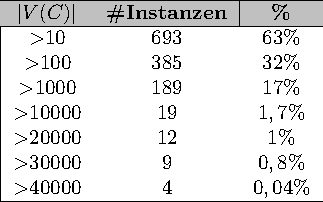
\includegraphics[width = 6cm]{pictures/compiled/instance_sizes_distribution_table}
		\caption{Visualisierung eines Matches über eine lange Kante}
		\label{bild:sizes_table}
	\end{wrapfigure}
 Abbildung \ref{bild:sizes_table} zeigt die Verteilung der getesteten Instanzen hinsichtlich der Größe  ihrer Knotenmenge.
 
\textcolor{red}{ Kandidaten menge kann hier noch hin also menge der Kandidaten abh von Knotenmenge bzw anzahl highfanoutknoten  und abh von den oben genannten zusatzfeatures (zb pinabh. delay, Library )  \\  und dass vielleicht die varianz (anhand eines bildes beweisen?) des hoghfanout anteil ziemlich klein ist und somit Knotenmenge und highfanoutmenge ansich ausreichend aussagekräftig sind} 
 
 \subsection{Analyse der Ergebnisse}
 \label{subsec:analyse_der_ergebnisse}
\textcolor{red}{irgendwo muss noch erwähnt werden, dass die größe/vt und at werte am anfang gleich gesetzt werden }
\subsubsection{Tradeoffparameter}

\subsubsection{Premapping}

\subsubsection{Präprozessing}
\textcolor{red}{inclusive der graphen größe vergleiche}

\subsubsection{Power und Area Vergleich}

\subsubsection{Bucket filetering $\epsilon$ im vergleich }

\subsubsection{Gütevergleich kleiner "optimal " gel instanzen}


\subsubsection{Verhalten weiterer Kosten}
\textcolor{red}{die anfallenden kosten die nicht im \TM gemessen werden beobachten und in der future work dran anschließen}

\subsubsection{Zusammenfassung?}
\textcolor{red}{oder am ende nur ein laufzeit güte tradeoff mit eigenem Unterkapitel ?} 
 
 
 \subsection{Laufzeitanalyse}
 \label{subsec:laufzeitanalyse}
Aus der theoretischen Laufzeitschranke aus Kapitel \ref{subsubsec:heuristik} folgt, dass die Laufzeit maßgeblich von der Menge der Highfanoutknoten abhängt. Andere Faktoren wie das Aufteilen von Gates, die Größe der Library oder die Wahl der Premapping subroutine spielen ebenfalls eine wichtige Rolle. Dies verdeutlicht die Übersicht \textcolor{red}{??}.\\
 Bezüglich der Größe der Library lassen sich die Chips, abzüglich weniger Unterschiede in zwei Gruppen einteilen. Die markierte Teilmenge der Abbildung \textcolor{red}{??} entspricht der Menge der (so genannten) komplexen Gates. Ein Chip lässt sich in der Praxis, abhängig davon ob er de komplexen Gates grundsätzlich erlaubt, einer der zwei Gruppen zuordnen. Diese Unterscheidung findet sich ebenfalls in Abbildung \textcolor{red}{??}.
 
\subsubsection{globale Laufzeitanalyse}
\textcolor{red}{welche größenordnungen sind überhaupt lösbar}

\subsubsection{locale Laufzeitanalyse}
\textcolor{red}{wie unterscheiden sich die einzelnen Varianten in der Laufzeit? \\ oder lässt sich beides gut in einem bild erkennen ?} \\

\textcolor{red}{hier auch die decompose laufzeit vgl mit rein ?}

\subsubsection{Bucket filetering $\epsilon$ im vergleich } 
 
\subsubsection{Laufzeitverlgeich kleiner "optimal " gel instanzen}


\subsection{Güte laufzeit vergleich}
\subsubsection{kleine Instanzen}

\subsubsection{allgemein}
\textcolor{red}{wahrscheinlich ist der unterschied bei decompose und ohne am größten den mit der besten premapping methode durchführen}

\subsubsection{Güte Bucket filetering $\epsilon$ }

\section{Fazit und Ausblick}
\label{sec:fazit_und_ausblick}
	







\newpage
%\clearpage

\end{document}
